% Options for packages loaded elsewhere
% Options for packages loaded elsewhere
\PassOptionsToPackage{unicode}{hyperref}
\PassOptionsToPackage{hyphens}{url}
\PassOptionsToPackage{dvipsnames,svgnames,x11names}{xcolor}
%
\documentclass[
  12pt,
  letterpaper,
  DIV=11,
  numbers=noendperiod]{scrartcl}
\usepackage{xcolor}
\usepackage[margin=.75in]{geometry}
\usepackage{amsmath,amssymb}
\setcounter{secnumdepth}{3}
\usepackage{iftex}
\ifPDFTeX
  \usepackage[T1]{fontenc}
  \usepackage[utf8]{inputenc}
  \usepackage{textcomp} % provide euro and other symbols
\else % if luatex or xetex
  \usepackage{unicode-math} % this also loads fontspec
  \defaultfontfeatures{Scale=MatchLowercase}
  \defaultfontfeatures[\rmfamily]{Ligatures=TeX,Scale=1}
\fi
\usepackage{lmodern}
\ifPDFTeX\else
  % xetex/luatex font selection
  \setmainfont[]{Times New Roman}
\fi
% Use upquote if available, for straight quotes in verbatim environments
\IfFileExists{upquote.sty}{\usepackage{upquote}}{}
\IfFileExists{microtype.sty}{% use microtype if available
  \usepackage[]{microtype}
  \UseMicrotypeSet[protrusion]{basicmath} % disable protrusion for tt fonts
}{}
\usepackage{setspace}
\makeatletter
\@ifundefined{KOMAClassName}{% if non-KOMA class
  \IfFileExists{parskip.sty}{%
    \usepackage{parskip}
  }{% else
    \setlength{\parindent}{0pt}
    \setlength{\parskip}{6pt plus 2pt minus 1pt}}
}{% if KOMA class
  \KOMAoptions{parskip=half}}
\makeatother
% Make \paragraph and \subparagraph free-standing
\makeatletter
\ifx\paragraph\undefined\else
  \let\oldparagraph\paragraph
  \renewcommand{\paragraph}{
    \@ifstar
      \xxxParagraphStar
      \xxxParagraphNoStar
  }
  \newcommand{\xxxParagraphStar}[1]{\oldparagraph*{#1}\mbox{}}
  \newcommand{\xxxParagraphNoStar}[1]{\oldparagraph{#1}\mbox{}}
\fi
\ifx\subparagraph\undefined\else
  \let\oldsubparagraph\subparagraph
  \renewcommand{\subparagraph}{
    \@ifstar
      \xxxSubParagraphStar
      \xxxSubParagraphNoStar
  }
  \newcommand{\xxxSubParagraphStar}[1]{\oldsubparagraph*{#1}\mbox{}}
  \newcommand{\xxxSubParagraphNoStar}[1]{\oldsubparagraph{#1}\mbox{}}
\fi
\makeatother


\usepackage{longtable,booktabs,array}
\usepackage{calc} % for calculating minipage widths
% Correct order of tables after \paragraph or \subparagraph
\usepackage{etoolbox}
\makeatletter
\patchcmd\longtable{\par}{\if@noskipsec\mbox{}\fi\par}{}{}
\makeatother
% Allow footnotes in longtable head/foot
\IfFileExists{footnotehyper.sty}{\usepackage{footnotehyper}}{\usepackage{footnote}}
\makesavenoteenv{longtable}
\usepackage{graphicx}
\makeatletter
\newsavebox\pandoc@box
\newcommand*\pandocbounded[1]{% scales image to fit in text height/width
  \sbox\pandoc@box{#1}%
  \Gscale@div\@tempa{\textheight}{\dimexpr\ht\pandoc@box+\dp\pandoc@box\relax}%
  \Gscale@div\@tempb{\linewidth}{\wd\pandoc@box}%
  \ifdim\@tempb\p@<\@tempa\p@\let\@tempa\@tempb\fi% select the smaller of both
  \ifdim\@tempa\p@<\p@\scalebox{\@tempa}{\usebox\pandoc@box}%
  \else\usebox{\pandoc@box}%
  \fi%
}
% Set default figure placement to htbp
\def\fps@figure{htbp}
\makeatother


% definitions for citeproc citations
\NewDocumentCommand\citeproctext{}{}
\NewDocumentCommand\citeproc{mm}{%
  \begingroup\def\citeproctext{#2}\cite{#1}\endgroup}
\makeatletter
 % allow citations to break across lines
 \let\@cite@ofmt\@firstofone
 % avoid brackets around text for \cite:
 \def\@biblabel#1{}
 \def\@cite#1#2{{#1\if@tempswa , #2\fi}}
\makeatother
\newlength{\cslhangindent}
\setlength{\cslhangindent}{1.5em}
\newlength{\csllabelwidth}
\setlength{\csllabelwidth}{3em}
\newenvironment{CSLReferences}[2] % #1 hanging-indent, #2 entry-spacing
 {\begin{list}{}{%
  \setlength{\itemindent}{0pt}
  \setlength{\leftmargin}{0pt}
  \setlength{\parsep}{0pt}
  % turn on hanging indent if param 1 is 1
  \ifodd #1
   \setlength{\leftmargin}{\cslhangindent}
   \setlength{\itemindent}{-1\cslhangindent}
  \fi
  % set entry spacing
  \setlength{\itemsep}{#2\baselineskip}}}
 {\end{list}}
\usepackage{calc}
\newcommand{\CSLBlock}[1]{\hfill\break\parbox[t]{\linewidth}{\strut\ignorespaces#1\strut}}
\newcommand{\CSLLeftMargin}[1]{\parbox[t]{\csllabelwidth}{\strut#1\strut}}
\newcommand{\CSLRightInline}[1]{\parbox[t]{\linewidth - \csllabelwidth}{\strut#1\strut}}
\newcommand{\CSLIndent}[1]{\hspace{\cslhangindent}#1}



\setlength{\emergencystretch}{3em} % prevent overfull lines

\providecommand{\tightlist}{%
  \setlength{\itemsep}{0pt}\setlength{\parskip}{0pt}}



 


\usepackage{etoolbox}
\AtBeginEnvironment{longtable}{\singlespacing}
\renewcommand{\arraystretch}{1.2}
\KOMAoption{captions}{tableheading}
\makeatletter
\@ifpackageloaded{caption}{}{\usepackage{caption}}
\AtBeginDocument{%
\ifdefined\contentsname
  \renewcommand*\contentsname{Table of contents}
\else
  \newcommand\contentsname{Table of contents}
\fi
\ifdefined\listfigurename
  \renewcommand*\listfigurename{List of Figures}
\else
  \newcommand\listfigurename{List of Figures}
\fi
\ifdefined\listtablename
  \renewcommand*\listtablename{List of Tables}
\else
  \newcommand\listtablename{List of Tables}
\fi
\ifdefined\figurename
  \renewcommand*\figurename{Figure}
\else
  \newcommand\figurename{Figure}
\fi
\ifdefined\tablename
  \renewcommand*\tablename{Table}
\else
  \newcommand\tablename{Table}
\fi
}
\@ifpackageloaded{float}{}{\usepackage{float}}
\floatstyle{ruled}
\@ifundefined{c@chapter}{\newfloat{codelisting}{h}{lop}}{\newfloat{codelisting}{h}{lop}[chapter]}
\floatname{codelisting}{Listing}
\newcommand*\listoflistings{\listof{codelisting}{List of Listings}}
\makeatother
\makeatletter
\makeatother
\makeatletter
\@ifpackageloaded{caption}{}{\usepackage{caption}}
\@ifpackageloaded{subcaption}{}{\usepackage{subcaption}}
\makeatother
\usepackage{bookmark}
\IfFileExists{xurl.sty}{\usepackage{xurl}}{} % add URL line breaks if available
\urlstyle{same}
\hypersetup{
  pdftitle={MSDM CEP Chapter 2 Development Progress Reports 1--5},
  pdfauthor={Group 9: Luis Ahumada, Spencer Conway, Carmen Jimenez Rodriguez, Leeann Lewis-Waddell, Georgia Monjarrez},
  colorlinks=true,
  linkcolor={blue},
  filecolor={Maroon},
  citecolor={Blue},
  urlcolor={Blue},
  pdfcreator={LaTeX via pandoc}}


\title{MSDM CEP Chapter 2 Development Progress Reports 1--5}
\usepackage{etoolbox}
\makeatletter
\providecommand{\subtitle}[1]{% add subtitle to \maketitle
  \apptocmd{\@title}{\par {\large #1 \par}}{}{}
}
\makeatother
\subtitle{Client: Restaurant at Kellogg Ranch}
\author{Group 9: Luis Ahumada, Spencer Conway, Carmen Jimenez Rodriguez,
Leeann Lewis-Waddell, Georgia Monjarrez}
\date{}
\begin{document}
\maketitle

\renewcommand*\contentsname{Table of contents}
{
\hypersetup{linkcolor=}
\setcounter{tocdepth}{3}
\tableofcontents
}

\setstretch{2}
\section{Progress Report 1}\label{progress-report-1}

\subsection{Evidence Search and Approach
Challenge}\label{evidence-search-and-approach-challenge}

\begin{itemize}
\tightlist
\item
  \href{https://drive.google.com/drive/folders/1du_W7r7T4k9v3Y39YWYY-aHQAu7HKRU8?usp=sharing}{Google
  Drive Containing Individual Reports}
\end{itemize}

\section{Progress Report 2}\label{progress-report-2}

\subsubsection{AO1. Newsletter Design and Reservation Growth (Leeann
Lewis-Waddell)}\label{sec-ao1-title-ao1}

\begin{longtable}[]{@{}
  >{\raggedright\arraybackslash}p{(\linewidth - 8\tabcolsep) * \real{0.1800}}
  >{\raggedright\arraybackslash}p{(\linewidth - 8\tabcolsep) * \real{0.2200}}
  >{\raggedright\arraybackslash}p{(\linewidth - 8\tabcolsep) * \real{0.2400}}
  >{\raggedright\arraybackslash}p{(\linewidth - 8\tabcolsep) * \real{0.1800}}
  >{\raggedright\arraybackslash}p{(\linewidth - 8\tabcolsep) * \real{0.1800}}@{}}
\caption{AO1 Model Comparison Table}\tabularnewline
\toprule\noalign{}
\begin{minipage}[b]{\linewidth}\raggedright
Approach / Model
\end{minipage} & \begin{minipage}[b]{\linewidth}\raggedright
What It Explains
\end{minipage} & \begin{minipage}[b]{\linewidth}\raggedright
Evidence for / Against
\end{minipage} & \begin{minipage}[b]{\linewidth}\raggedright
Data / Assumptions
\end{minipage} & \begin{minipage}[b]{\linewidth}\raggedright
Fit with AO
\end{minipage} \\
\midrule\noalign{}
\endfirsthead
\toprule\noalign{}
\begin{minipage}[b]{\linewidth}\raggedright
Approach / Model
\end{minipage} & \begin{minipage}[b]{\linewidth}\raggedright
What It Explains
\end{minipage} & \begin{minipage}[b]{\linewidth}\raggedright
Evidence for / Against
\end{minipage} & \begin{minipage}[b]{\linewidth}\raggedright
Data / Assumptions
\end{minipage} & \begin{minipage}[b]{\linewidth}\raggedright
Fit with AO
\end{minipage} \\
\midrule\noalign{}
\endhead
\bottomrule\noalign{}
\endlastfoot
Email Response Process (Hartemo, Suomi, and Hakala 2016; Kumar 2021) &
How readers move from viewing a newsletter to clicking and eventually
purchasing. & Hartemo, Suomi, and Hakala (2016) tested newsletter
formats against a control, and Kumar (2021) found clicks had the
strongest link to purchases. Both studies were conducted in commercial
settings rather than a university newsletter. & Requires page views,
clicks, and reservation data. Assumes each stage can be measured
separately. & Strongest overall fit because it matches the stages Canva
and OpenTable can measure. \\
Visual Attention and Heuristics (Kumar and Salo 2018; Skourou and
Spiliotopoulos 2024) & Where readers look in a newsletter and which
elements they are most likely to click. & Kumar and Salo (2018) found
upper-left links earn higher click-through rates, and Skourou and
Spiliotopoulos (2024) found large images capture attention. Images may
also pull attention away from the button. & Requires versions that
differ in button placement or media while all other elements stay the
same. & Good fit for choosing the test variables, but does not connect
clicks to reservations. \\
Cognitive Load and Information Overload (Bashirzadeh, Mai, and Faure
2022; Kong, Zhu, and Konstan 2021) & Why adding too much content, or
sending too many emails, can reduce engagement. & Bashirzadeh, Mai, and
Faure (2022) found combining visual elements increased unsubscribes, and
Kong, Zhu, and Konstan (2021) found university recipients often ignore
bulk email. & Requires page views alongside clicks to separate a design
problem from a readership problem. & Useful boundary condition, but
explains limits rather than what drives clicks. \\
Industry Best Practices (Go 2024; Jones 2023) & Practical
recommendations for email design and benchmark click-through rates. &
Both guides recommend strong visuals, bold CTAs near the top, and
testing one variable at a time. Both are written by companies that sell
marketing or reservation services. & Assumes general benchmarks apply to
RKR's audience. & Helpful for benchmarks, but too weak to serve as the
main framework. \\
\end{longtable}

The Email Response Process is the strongest fit for AO1 because it
follows readers from viewing the newsletter to clicking the ``Reserve a
Table'' button to making a reservation. This sequence matches the data
available through Canva and OpenTable, which allows each stage to be
measured. Visual attention research supports the decision to test button
placement and media, while cognitive load research explains why only one
change will be tested at a time. As such, the combination of these
frameworks fits AO1 better than relying on industry best practices
alone.

The evidence shows that button placement and visual design both affect
click-through rate, and that clicks are closely connected to purchases.
What remains uncertain is whether these findings will hold for a
university audience that may already be overwhelmed by bulk email. It is
also unclear whether the mailing list can be segmented and whether
OpenTable can attribute reservations to separate links. Since two of my
teammates are analyzing Facebook and Instagram, this analysis will focus
only on the newsletter and should not assume it is the only channel
influencing reservations. AO1 was already revised to test button
placement in Fall and media in Spring, so no further revision is needed
at this stage.

\subsubsection{AO2. Customer Experience Factors Associated With Overall
Satisfaction (Carmen
Jimenez)}\label{ao2.-customer-experience-factors-associated-with-overall-satisfaction-carmen-jimenez}

\begin{longtable}[]{@{}
  >{\raggedright\arraybackslash}p{(\linewidth - 8\tabcolsep) * \real{0.1800}}
  >{\raggedright\arraybackslash}p{(\linewidth - 8\tabcolsep) * \real{0.2200}}
  >{\raggedright\arraybackslash}p{(\linewidth - 8\tabcolsep) * \real{0.2400}}
  >{\raggedright\arraybackslash}p{(\linewidth - 8\tabcolsep) * \real{0.1800}}
  >{\raggedright\arraybackslash}p{(\linewidth - 8\tabcolsep) * \real{0.1800}}@{}}
\caption{AO2 Model Comparison Table}\tabularnewline
\toprule\noalign{}
\begin{minipage}[b]{\linewidth}\raggedright
Approach / Model
\end{minipage} & \begin{minipage}[b]{\linewidth}\raggedright
What It Explains
\end{minipage} & \begin{minipage}[b]{\linewidth}\raggedright
Evidence for / Against
\end{minipage} & \begin{minipage}[b]{\linewidth}\raggedright
Data / Assumptions
\end{minipage} & \begin{minipage}[b]{\linewidth}\raggedright
Fit with AO
\end{minipage} \\
\midrule\noalign{}
\endfirsthead
\toprule\noalign{}
\begin{minipage}[b]{\linewidth}\raggedright
Approach / Model
\end{minipage} & \begin{minipage}[b]{\linewidth}\raggedright
What It Explains
\end{minipage} & \begin{minipage}[b]{\linewidth}\raggedright
Evidence for / Against
\end{minipage} & \begin{minipage}[b]{\linewidth}\raggedright
Data / Assumptions
\end{minipage} & \begin{minipage}[b]{\linewidth}\raggedright
Fit with AO
\end{minipage} \\
\midrule\noalign{}
\endhead
\bottomrule\noalign{}
\endlastfoot
Multidimensional Restaurant Quality Framework (Ryu, Lee, and Kim 2012) &
Explains how food quality, service quality, and the physical environment
relate to customer satisfaction and behavioral intentions. & Ryu, Lee,
and Kim (2012) support evaluating several restaurant-quality dimensions
together. The original restaurant context differs from RKR. & Requires
guest ratings of food quality, service quality, physical environment,
and satisfaction. Assumes guests can evaluate these dimensions
separately. & Strongest overall fit because it directly includes the
three main experience dimensions measured in AO2. \\
Food Quality--Satisfaction Approach (Namkung and Jang 2007) & Explains
how food quality relates to customer satisfaction and behavioral
intentions. & Namkung and Jang (2007) support food quality as an
important part of restaurant satisfaction. The approach focuses mainly
on food rather than the entire dining experience. & Requires guest
ratings of food-related characteristics such as quality, presentation,
enjoyment, and consistency. & Good fit for the food-quality component of
AO2, but too narrow to address the full objective alone. \\
Physical Environment / Atmospherics Approach (Han and Ryu 2009; Heung
and Gu 2012) & Explains how atmosphere and the physical environment
relate to satisfaction and behavioral responses. & Han and Ryu (2009)
and Heung and Gu (2012) support the importance of the restaurant
environment. This approach does not fully account for food or service
quality. & Requires guest evaluations of atmosphere and
physical-environment characteristics such as cleanliness, comfort,
décor, layout, and overall ambiance. & Good fit for the atmosphere and
physical-environment component, but not sufficient by itself to address
AO2. \\
Customer Satisfaction--Behavioral Intentions Approach (Arora and Singer
2006) & Explains how customer satisfaction relates to future intentions
such as returning to or recommending a restaurant. & Research supports a
relationship between satisfaction and behavioral intentions, but stated
intentions do not confirm actual future behavior. & Requires measures of
overall satisfaction, intention to return, and willingness to recommend.
& Useful secondary fit because AO2 includes return intention and
recommendation, but it does not directly identify the strongest and
weakest experience areas. \\
\end{longtable}

The Multidimensional Restaurant Quality Framework is the strongest fit
for AO2 because it directly includes the three main experience
dimensions measured in this objective: food quality, service quality,
and the physical environment. Ryu, Lee, and Kim (2012) show that these
dimensions are connected to customer satisfaction and behavioral
intentions. This framework is broader than the food-quality and
physical-environment approaches because it allows the dining experience
to be evaluated as a combination of multiple factors rather than
focusing on only one area.

The existing research shows that food quality, service quality, and
atmosphere or physical environment are important parts of the restaurant
experience. However, the literature cannot determine which of these
areas RKR guests rate most positively or negatively. This is especially
important because RKR is a student-operated restaurant located on a
university campus, which may create a different guest experience from
the restaurants studied in previous research. For this reason, AO2 still
requires primary survey data from RKR guests. The current AO does not
need to be revised because it is measurable, directly connected to the
available survey data, and aligned with the project objective of
identifying strengths and improvement opportunities in the RKR dining
experience.

\subsubsection{AO3 Facebook Content and Messaging Strategies and
Reservation
Performance}\label{ao3-facebook-content-and-messaging-strategies-and-reservation-performance}

\begin{longtable}[]{@{}
  >{\raggedright\arraybackslash}p{(\linewidth - 8\tabcolsep) * \real{0.1800}}
  >{\raggedright\arraybackslash}p{(\linewidth - 8\tabcolsep) * \real{0.2200}}
  >{\raggedright\arraybackslash}p{(\linewidth - 8\tabcolsep) * \real{0.2400}}
  >{\raggedright\arraybackslash}p{(\linewidth - 8\tabcolsep) * \real{0.1800}}
  >{\raggedright\arraybackslash}p{(\linewidth - 8\tabcolsep) * \real{0.1800}}@{}}
\caption{AO3 Model Comparison Table}\tabularnewline
\toprule\noalign{}
\begin{minipage}[b]{\linewidth}\raggedright
Approach/Model
\end{minipage} & \begin{minipage}[b]{\linewidth}\raggedright
What It Explains
\end{minipage} & \begin{minipage}[b]{\linewidth}\raggedright
Evidence for/Against
\end{minipage} & \begin{minipage}[b]{\linewidth}\raggedright
Data/Assumptions
\end{minipage} & \begin{minipage}[b]{\linewidth}\raggedright
Fit with AO
\end{minipage} \\
\midrule\noalign{}
\endfirsthead
\toprule\noalign{}
\begin{minipage}[b]{\linewidth}\raggedright
Approach/Model
\end{minipage} & \begin{minipage}[b]{\linewidth}\raggedright
What It Explains
\end{minipage} & \begin{minipage}[b]{\linewidth}\raggedright
Evidence for/Against
\end{minipage} & \begin{minipage}[b]{\linewidth}\raggedright
Data/Assumptions
\end{minipage} & \begin{minipage}[b]{\linewidth}\raggedright
Fit with AO
\end{minipage} \\
\midrule\noalign{}
\endhead
\bottomrule\noalign{}
\endlastfoot
Processing Fluency (Philp, Jacobson, and Pancer 2022a) & Why clear and
recognizable visual content may be easier for customers to process and
respond to & Recognizable food images received stronger engagement but
does not explain rservatin & Posts have to be grouped by visuall/content
characteristics and compared using engagement metrics. & Good fit for
explaining visual content performance but not enough for the full AO \\
Media Richness+Speech Act Theory (Manningham, Asselin, and Bourguignon
2024) & How wording, format, and message presentation might affect
engagement & Direct wording and emoji use were linked to higher
restaurant Facebook engagement & Posts would need to be coded by message
style, wording, and format. & Good fit for messaging section of AO but
not the reservation part \\
Digital Consumer Engagement+Customer Behavioral Response

{[}Halloran and Lutz (2021); (Yost, Zhang, and Qi 2021) & How customers
engage with Facebook content and how that engagement can be related to
customer behavior & Stronger engagement was linked to purchase frequency
and sales. & Would need Facebook engagement and a downstream behavioral
measurement like OpenTable activity & Overall this would be the best fit
because AO3 is examining Facebook engagement and reservation-related
behavior \\
Theory of Reasoned Act/Customer Journey

{[}Hanaysha (2022); (Veloso and Gomez-Suarez 2023) & How customers might
move from engagement stage to the action stage & Engagement was linked
to purchase intention but intention is not an actual measurable behavior
& This assumes that outside factors might exist between the initial
engagement stage to the reservation stage. & Weaker than the others for
analyzing reservation acitivity \\
\end{longtable}

Digital Consumer Engagement and Customer Behavioral Response are the
strongest fits for AO3 because they are directly connected to Facebook
engagement with downstream behavior. Digital Consumer Engagement helps
explain how customers react to different Facebook content and messaging,
while Behavioral Response helps connect the initial engagement to an
action that is taken later like making a reservation or visiting the
RKR. This combination fits AO3 better than the others because they are
more useful for explaining why specific posts perform better, and
intention, but don't explain the following steps in the customer
journey.

The evidence show that Facebook content, visual presentation, and
messaging style can influence customer engagement. It also shows that
some forms forms of engagement might be connected to customer behavior.
What is uncertain is whether Facebook strategies that perform better for
RKR will be connected to stronger OpenTable reservation activity. One
thing to also keep in mind is that two of my group members are analyzing
Instagram and the newsletter, so this analysis will only focus on
Facebook and should not assume that Facebook is the only channel
influencing reservation. At this point, AO3 does not need to be revise
because it fits the overall project and available research.

\subsubsection{AO4 Website Content Navigation and Usability (Georgia
Monjarrez)}\label{ao4-website-content-navigation-and-usability-georgia-monjarrez}

\begin{longtable}[]{@{}
  >{\raggedright\arraybackslash}p{(\linewidth - 8\tabcolsep) * \real{0.1800}}
  >{\raggedright\arraybackslash}p{(\linewidth - 8\tabcolsep) * \real{0.2200}}
  >{\raggedright\arraybackslash}p{(\linewidth - 8\tabcolsep) * \real{0.2400}}
  >{\raggedright\arraybackslash}p{(\linewidth - 8\tabcolsep) * \real{0.1800}}
  >{\raggedright\arraybackslash}p{(\linewidth - 8\tabcolsep) * \real{0.1800}}@{}}
\toprule\noalign{}
\begin{minipage}[b]{\linewidth}\raggedright
Approach / Model
\end{minipage} & \begin{minipage}[b]{\linewidth}\raggedright
What It Explains
\end{minipage} & \begin{minipage}[b]{\linewidth}\raggedright
Evidence for / Against
\end{minipage} & \begin{minipage}[b]{\linewidth}\raggedright
Data / Assumptions
\end{minipage} & \begin{minipage}[b]{\linewidth}\raggedright
Fit with AO
\end{minipage} \\
\midrule\noalign{}
\endhead
\bottomrule\noalign{}
\endlastfoot
Selected DeLone and McLean constructs (DeLone and McLean 2003) &
Separates information/system quality visitor responses and benefits. &
Broad established framework. does not prove effects of RKR changes. &
Content and navigation review feedback defined use outcomes. full model
testing requires adequate measures and sample. & Organizing framework
with task performance as the project outcome. \\
Technology acceptance and hospitality information quality (Davis 1989;
Jeong and Lambert 2001) & Distinguishes perceived ease usefulness and
information quality. & Supports separate visitor perceptions. original
technology and simulated hotel contexts limit transfer. & Adapted
five-point ease item and optional usefulness feedback. adapted items are
not the complete validated scales. & Useful supplement. perceptions
alone cannot establish the 80\% completion target. \\
DINEWEBQUAL and information-task fit (Dedeke 2016; Kim et al. 2012) &
Restaurant-specific quality and information relevant to tasks. &
Restaurant dimensions supported in 211 students. travel context supports
task fit. Intentions do not establish bookings. & Review categories and
feedback on menu/hours/reservation tasks. adaptations require caution. &
Guides content and quality diagnosis alongside task observation. \\
Task-based usability evaluation (Hornbæk 2006; Hornbæk and Law 2007;
Tuch et al. 2012) & Whether visitors complete tasks time needed and
experienced difficulty. & Supports distinct performance and perception
measures. small samples limit generalization and appearance is
insufficient. & Completion counts/rates median time for successful
unassisted attempts and five-point ease distributions. defined endpoints
and recorded devices/familiarity. & Principal method for evaluating each
task against the proposed 80\% target. selected accessibility checks
supplement it. \\
\end{longtable}

AO4 Model Comparison Table

\subsubsection{AO5 Instagram Content Format and Engagement (Spencer
Conway)}\label{ao5-instagram-content-format-and-engagement-spencer-conway}

\begin{longtable}[]{@{}
  >{\raggedright\arraybackslash}p{(\linewidth - 8\tabcolsep) * \real{0.1800}}
  >{\raggedright\arraybackslash}p{(\linewidth - 8\tabcolsep) * \real{0.2200}}
  >{\raggedright\arraybackslash}p{(\linewidth - 8\tabcolsep) * \real{0.2400}}
  >{\raggedright\arraybackslash}p{(\linewidth - 8\tabcolsep) * \real{0.1800}}
  >{\raggedright\arraybackslash}p{(\linewidth - 8\tabcolsep) * \real{0.1800}}@{}}
\toprule\noalign{}
\begin{minipage}[b]{\linewidth}\raggedright
Approach / Model
\end{minipage} & \begin{minipage}[b]{\linewidth}\raggedright
What It Explains
\end{minipage} & \begin{minipage}[b]{\linewidth}\raggedright
Evidence for / Against
\end{minipage} & \begin{minipage}[b]{\linewidth}\raggedright
Data / Assumptions
\end{minipage} & \begin{minipage}[b]{\linewidth}\raggedright
Fit with AO
\end{minipage} \\
\midrule\noalign{}
\endhead
\bottomrule\noalign{}
\endlastfoot
\begin{minipage}[t]{\linewidth}\raggedright
Stimulus--Organism--Response (S--O--R) Framework\\
(Bushara et al. 2023)\strut
\end{minipage} & How social media content can affect what people think
and how they respond. & Restaurant research supports connections between
social media marketing, perceived value, and behavioral intentions. It
does not show which Instagram format gets the most engagement. & Would
need audience feedback to measure perceptions, along with engagement
data. Assumes those perceptions help explain the response. & Good
support for explaining audience responses, but Instagram Insights cannot
test the whole framework. \\
Processing Fluency {[}(Philp, Jacobson, and Pancer 2022b){]} & Why clear
and recognizable food images may be easier to understand and engage
with. & Typical-looking food images were linked to stronger engagement,
but this does not tell us whether Reels, carousels, or single images
work best. & Posts would need to be grouped by visual characteristics
and compared using engagement metrics. Audience feedback would be needed
to test the explanation directly. & Helpful for the visual content part
of the AO, but not enough to answer the full objective. \\
Uses and Gratifications Theory (Kulikovskaja et al. 2023) & Why people
engage with content that provides information, entertainment, or social
connection. & Restaurant research connects different content types with
engagement. However, findings from other platforms may not apply
directly to RKR's Instagram. & Posts would need to be grouped by content
purpose as well as format. Assumes people choose content that meets
their needs; audience feedback would help confirm those motivations. &
Useful for explaining why people respond to content, but does not
identify the strongest format by itself. \\
Post-Format Comparison and Content Testing & Which Instagram formats get
stronger engagement for RKR. & Directly addresses the AO, but
differences could also come from the topic, posting time, or paid
promotion. & Requires post format, reach, likes, comments, shares, and
saves. Posts need similar measurement windows and reasonably similar
posting conditions. & Best overall fit because AO5 looks at past posts
and then tests new content in selected formats. \\
\end{longtable}

AO5 Model Comparison Table

Post-format comparison with support from S--O--R and Uses and
Gratifications is the best fit for AO5. Comparing formats will help us
see whether Reels, carousels, or single-image posts get stronger
engagement for RKR. S--O--R helps explain how content might affect
audience responses. Uses and Gratifications adds another explanation by
looking at what people get from the content, such as information,
entertainment, or social connection. Processing fluency helps explain
why some food images may perform better. These theories do not tell us
which format is best for RKR, so we still need to look at the account's
actual results. Past posts will be grouped by format to create a
baseline, and new posts will be compared with those results. Engagement
rate will be calculated using likes, comments, shares, and saves divided
by reach, multiplied by 100.

The research suggests that both visual presentation and content purpose
can affect engagement. Kulikovskaja et al.~(2023) found different
engagement patterns for informational and entertaining, reward-based,
and relationship-focused restaurant content. However, the research does
not establish what works best for RKR's Instagram audience. We will need
Instagram Insights data and information about each post's topic,
purpose, posting date, and whether it was promoted. For example, a Reel
might perform better because it is entertaining, rather than just
because it is a video. New posts should be measured over the same amount
of time so the comparison is more useful. Stronger engagement also does
not automatically mean more reservations. At this point, AO5 does not
need a major revision, although adding ``among the formats tested''
would make it more specific. We still need faculty guidance on how far
back to look at past posts and how many new posts to test.

\subsection{Investigation of Currently Available Research
Framework/Model}\label{investigation-of-currently-available-research-frameworkmodel}

\subsubsection{AO1. Newsletter Design and Reservation Growth (Leeann
Lewis-Waddell)}\label{ao1.-newsletter-design-and-reservation-growth-leeann-lewis-waddell}

\textbf{Analytics Objective:} Compare ``Reserve a Table'' click rates
and attributed OpenTable reservations across RKR newsletter section
designs, testing button placement in Fall 2026 and image versus video in
Spring 2027.

\paragraph{Existence of Well-established
Models}\label{existence-of-well-established-models}

Analytics Objective 1 intends to A/B test revisions of the current
advertising for the Restaurant at Kellogg Ranch within The Collins
Concierge, the department's weekly newsletter. Specifically, it will
test if an image-based or video-based ad will increase ``Reserve a
Table'' clicks in comparison to the current text-only format. After
extensive research, three established frameworks inform how that test
will be built and executed. AO1 will examine the email response process,
visual attention and heuristics, and cognitive load and information
overload.

Email marketing response occurs in a sequence, wherein a reader first
sees a message, engages with it, and then chooses whether to act on it.
Hartemo's newsletter testing model focuses on this response process,
linking the factors that affect response to the metrics that measure
each step (Hartemo, Suomi, and Hakala 2016). This study tests eight
format variations against a control group. The format of this analysis
easily applies directly to the comparison of image and video templates
against RKR's current section, which employs a controlled format test
with a no-graphic baseline.

A review of Kumar's framework divides newsletter success into relational
metrics, such as opens and clicks, and transactional metrics, such as
purchases (Kumar 2021). Drawing on 811 newsletters sent to 19,678
loyalty program members, the study determines that design significantly
shaped response, and clicks had the strongest relationship to eventual
purchase (Kumar 2021). This point supports using click-through rate as
AO1's primary metric, with reservations as the secondary, validating
measure. With respect to RKR, Kumar's sequence would apply to three
measurable stages: newsletter views in Canva, ``Reserve a Table''
clicks, and OpenTable reservations.

One point of note: the response process also exposes a gap AO1 has to
account for. Since RKR welcomes walk-ins and accepts Bronco Bucks, some
readers will move from acknowledging the new template section and move
directly to a visit without ever clicking. Therefore, version-specific
links or perhaps a ``How did you hear about us?'' question at booking
help capture that path, but would require additional points in the
customer journey to address this variable.

As can be expected, readers do not scan a newsletter evenly or in its
entirety. Described in detail by Kumar, visual heuristics guide where
the eye lands and subsequently what gets clicked. This study details how
newsletter readers follow a U-shaped pattern rather than the Z-pattern
typical of web pages. It also outlines how the upper-left region
produces higher CTR than links placed elsewhere (Kumar and Salo 2018).
In the current RKR section, ``view the menu'' is a clickable link at the
top center while the ``Reserve a Table'' button sits at the bottom,
below the hours. Because placement carries its own documented effect,
both test versions keep the button in the same position; otherwise a
change in clicks could come from placement rather than media. Using
current metrics as a baseline, AO1 will test relocation of the clickable
``Reserve a Table'' button for the remainder of the fall, and media
additions through the sixteen weeks of Spring.

With regard to adding media to the RKR section of The Collins Concierge,
Imagery is known to compete strongly for attention once an email is
open. Skourou's study using eye-tracking technique and tools found that
large images captured more attention than discount codes and prices in
promotional emails. Notably, what readers chose to look at mapped to
their purchase decisions (Skourou and Spiliotopoulos 2024). This
supports visual content as AO1's main test variable, since the current
section depends on a block of text to communicate its key details,
specifically food and its accompanying atmosphere. On the contrary, the
study also shows that a strong image or video could consequently draw
focus away from the button it is meant to support.

Industry guides from Semrush and OpenTable support the aforementioned
notion. High-quality images are most recommended, coupled with
contrasting CTAs, and testing one variable at a time over at least two
weeks (Go 2024). OpenTable's restaurant guide adds that key information
belongs at the top, supported by strong food photos and bold CTA buttons
(Jones 2023). For RKR, Chef Matt's seasonal dishes offer natural subject
matter for either format.

This objective intends to be mindful of the potential for cognitive
overload and the possibility to annoy or turn-off the target audience.
Visual content can compete for a reader's limited attention rather than
enhance or entice. A large field experiment found that while GIFs and
emojis did not affect CTR individually, combining them inadvertently
increased unsubscribes, as the elements competed for the same cognitive
resources (Bashirzadeh, Mai, and Faure 2022). As such, AO1 aims to add
only one visual element at a time. The image and video templates will
match in layout, copy, and button placement, making media the only
variable.

Research for this objective also flags the potential for inbox overload.
Several studies found university recipients reported receiving 30 bulk
emails in a single week, often opening them without reading and trashing
22\% of newsletters (Kong, Zhu, and Konstan 2021). At one business
school, academics received 324 organizational bulk emails in a single
year with no option to unsubscribe (Bicudo De Castro 2025). As such, if
Collins Concierge readers are facing similar volume in addition to
academic workload, this objective must acknowledge that a redesign may
not move CTR regardless of format. This is why AO1 measures clicks per
view directly rather than relying on open rates.

Email also struggles when it lacks a clear role in the audience's
decision process. Survey respondents reacted with resistance and
irritation toward email marketing that did not fit their customer
journey (Zunac, Miletic, and Kozina 2022). The results of this study
justify treating the redesign as one input toward reservations rather
than its sole driver.

\paragraph{Adequateness of Gathered
Information}\label{adequateness-of-gathered-information}

The information above is significantly adequate in addressing the low
click-rate of RKR's newsletter channel. It addresses the potential
roadblocks in attracting the attention need to gain awareness, which is
overall design and aesthetics, particularly as it relates to the
placement of the desired goal, which it button location, but also
fatigue since the section does not change and does not employ
eye-catching media. On the other hand, it raises red flags with regard
to extenuating circumstances which may supercede the design
optimization, which are out of RKR's control such as inbox overload. The
studies align with industry suggestions, all of which are actionable and
applicable to the business problem. The only biases are really in the
industry guides from Semrush and OpenTable, since they are businesses
providing free resources to sway readers into purchasing services (Go
2024), (Jones 2023). Additionally, the eye-tracking study had a very
small pool of participants, and the Zunac study of the effectiveness of
email as a single marketing channel was largely comprised of female
participants, making the data somewhat biased (Skourou and
Spiliotopoulos 2024), (Zunac, Miletic, and Kozina 2022). This research
will be applied to revising the RKR section of The Collins Concierge, by
addressing button placement and aesthetics. Beginning with a baseline of
the previous issue's metrics, Fall will test only relocation of the
button to the upper left, and Spring will A/B test video versus image.

\paragraph{Need for Additional
Analysis}\label{need-for-additional-analysis}

Since the gathered information was largely sufficient but missing data
specific to the Concierge's audience, additional analysis is needed to
fully address the AO. None of the reviewed studies looked at a
restaurant section inside a university newsletter, so primary data will
fill that gap. Beginning with a baseline of CTR from previous Concierge
issues pulled from Canva, Fall will measure the effect of moving the
``Reserve a Table'' button to the upper left of the current text-only
section, and Spring will A/B test image versus video, alternating weekly
with the button in the same position. Page views will be tracked
alongside clicks, since the university studies suggest inbox overload
could keep readers from ever reaching the RKR section; this will help
determine whether low CTR is a design problem or a readership problem
(Kong, Zhu, and Konstan 2021), (Bicudo De Castro 2025). Each version
will also use its own link to OpenTable so reservations can be tied back
to the format that drove them. On the other hand, clicks will not
capture everyone, particularly guests who walk in or pay with Bronco
Bucks, so a ``How did you hear about us?'' question at booking will help
account for those visits. Holidays, finals, and campus events will be
noted throughout, since alternating weekly means outside factors could
affect results. Click rates between versions will be compared using a
two-proportion test to confirm whether differences are meaningful.

\paragraph{Assessment and Affirmation of Analytics
Objectives}\label{assessment-and-affirmation-of-analytics-objectives}

The original AO set out to A/B test two RKR section formats in The
Collins Concierge from October 2026 to June 2027, comparing ``Reserve a
Table'' click rates and attributed OpenTable reservations between
versions. It still holds, but the research has narrowed it, particularly
as it relates to what is being tested and when. It addresses RKR's need
to build sustainable demand by improving a section that is currently
easy to scroll past, with no imagery and a button placed at the bottom,
below the hours. On the other hand, testing media and button placement
at the same time would make it impossible to know which change caused an
increase, so the AO will be split into two phases. Two other approaches
were considered. A factorial test would compare every combination of
button placement and media at once {[}@hartemo2016{]}. However, it would
require splitting the mailing list into four groups, leaving too few
issues per version within one semester. A bundled redesign would be
simpler, but it would not show which change made the difference. As
such, the two-phase approach is the most practical option for isolating
one change at a time. Beginning with a baseline of CTR from previous
issues, Fall will test only the relocation of the button to the upper
left, and Spring will A/B test video versus image, alternating weekly
with the button in the same position. Canva will be used to track page
views and clicks, which is necessary for separating a design problem
from a readership problem, and each version will use its own link to
OpenTable to tie reservations back to the format. A two-proportion test
will compare click rates between versions, since it is a simple and
appropriate way to determine whether a difference is real or due to
chance. These tools are appropriate because they are already available
to RKR and the Concierge team, they require no individual reader data,
and they follow the same steps a reader takes from viewing the
newsletter to clicking to booking (Hartemo, Suomi, and Hakala 2016).

\subsubsection{AO2. Customer Experience Factors Associated With Overall
Satisfaction (Carmen
Jimenez)}\label{ao2.-customer-experience-factors-associated-with-overall-satisfaction-carmen-jimenez-1}

\textbf{Analytics Objective:} Using anonymous post-visit survey
responses, compare RKR guests' ratings of food quality, service quality,
and atmosphere/physical environment to identify the strongest and
weakest experience areas.

\paragraph{Existence of Well-established
Models}\label{existence-of-well-established-models-1}

Customer satisfaction is generally understood as a guest's overall
evaluation of a dining experience. In restaurant settings, this
evaluation is usually influenced by several parts of the experience
rather than by one factor alone. For AO2, the most relevant dimensions
are food quality, service quality, and atmosphere or the physical
environment. These dimensions provide a useful framework for
understanding what RKR guests value most and where improvements may be
needed.

A strong framework for AO2 comes from Ryu, Lee, and Kim, who examined
how food quality, service quality, and the physical environment
contribute to restaurant image, perceived value, customer satisfaction,
and behavioral intentions (Ryu, Lee, and Kim 2012). This framework is
especially useful for AO2 because it brings together the three main
experience dimensions that RKR plans to measure. Instead of evaluating
the dining experience only through food or only through service, the
framework treats the restaurant experience as multidimensional. This
supports the structure of the RKR survey and allows the team to compare
different parts of the guest experience using the same rating scale.

For RKR, this multidimensional approach is important because the
restaurant experience includes more than the meal itself. Guests
interact with the food, the service staff, and the restaurant
environment during the same visit. A guest may rate one of these areas
very positively while rating another area less favorably. Looking at the
dimensions separately can therefore provide more useful information than
relying only on one overall satisfaction question. The framework also
supports the use of overall satisfaction as a broader measure that can
be considered alongside the individual experience dimensions.

Food quality is one of the most established components of restaurant
satisfaction. Namkung and Jang found that food quality is associated
with customer satisfaction and behavioral intentions in restaurant
settings (Namkung and Jang 2007). Food quality can include
characteristics such as taste, freshness, presentation, temperature,
portion size, and consistency. These characteristics help explain why
food should be evaluated as its own part of the dining experience rather
than being combined with service or atmosphere.

This approach is relevant to AO2 because the survey can ask RKR guests
to evaluate their perception of the food experience directly. Ratings of
food quality can then be compared with ratings of service quality and
atmosphere or physical environment. If food receives the highest average
ratings, it may represent a current strength of the restaurant. If it
receives lower ratings than the other experience areas, the results may
identify an opportunity for improvement. However, the food-quality
approach alone is too narrow to fully address AO2 because the objective
examines the overall dining experience through several dimensions.

Service quality is another important component of restaurant customer
satisfaction. Ryu, Lee, and Kim's framework treats service quality
separately from food quality and the physical environment (Ryu, Lee, and
Kim 2012). This distinction is useful because a guest can enjoy the food
while still having a less positive experience with service, or the
opposite. Service quality may involve friendliness, attentiveness,
responsiveness, professionalism, communication, and reliability.

Service quality is particularly relevant to RKR because the restaurant
operates within The Collins College of Hospitality Management and also
functions as a learning environment. Guests are still customers of the
restaurant and evaluate the service they receive as part of their dining
experience. Measuring service quality separately can help RKR identify
whether guests view service as one of the strongest parts of the
experience or whether certain aspects may need attention. For AO2,
service ratings will therefore be compared with food-quality and
atmosphere ratings rather than being interpreted in isolation.

Atmosphere and the physical environment represent another established
area of restaurant research. Han and Ryu examined relationships among
the physical environment, price perception, customer satisfaction, and
restaurant loyalty (Han and Ryu 2009). Heung and Gu also examined the
influence of restaurant atmospherics on customer evaluations and
behavioral responses (Heung and Gu 2012). Together, these studies
support including the physical environment as a separate dimension of
the dining experience.

The physical environment may include elements such as cleanliness,
décor, lighting, seating, layout, comfort, and the overall atmosphere
created by the restaurant. For RKR, this dimension may also reflect the
restaurant's campus setting and the overall feeling guests experience
during lunch or dinner service. These elements are different from the
food and service themselves, but they can still contribute to how guests
evaluate the visit.

The physical-environment approach is useful for AO2 because it allows
RKR to identify whether the atmosphere is evaluated as positively as the
food and service. However, similar to the food-quality approach, it is
not sufficient by itself to answer the full analytics objective. AO2
requires a broader comparison of several experience dimensions. For this
reason, the multidimensional restaurant-quality framework provides a
stronger overall foundation, while the food-quality and
physical-environment approaches provide additional support for
individual dimensions.

Previous restaurant research also connects customer satisfaction with
future behavioral intentions, including intention to return and
willingness to recommend a restaurant (Arora and Singer 2006). These
measures are relevant to the RKR project because positive dining
experiences may contribute to repeat visits and positive
recommendations. However, AO2 will treat intention to return and
willingness to recommend as secondary descriptive indicators rather than
as evidence of actual future behavior. A guest stating that they intend
to return does not confirm that a repeat visit will actually occur.

Perceived value also appears in several restaurant models, including the
framework used by Ryu, Lee, and Kim (Ryu, Lee, and Kim 2012). However,
perceived value will not be treated as a primary dimension in the
current AO2. The revised objective is intentionally focused on food
quality, service quality, and atmosphere or physical environment.
Keeping these three dimensions as the main areas of comparison makes the
objective more focused and directly connected to the planned survey.

Taken together, the existing research provides a strong conceptual
foundation for AO2. The multidimensional restaurant-quality framework is
the strongest overall fit because it directly includes the three
experience dimensions that RKR plans to compare. The food-quality and
physical-environment approaches provide additional support for
understanding individual parts of the guest experience. These models
will guide the design of the anonymous post-visit survey and the
interpretation of the results.

The survey will use five-point rating items to measure food quality,
service quality, atmosphere and physical environment, overall
satisfaction, intention to return, and willingness to recommend.
Open-ended questions will also allow guests to identify the best part of
their experience and areas that could be improved. The existing research
therefore helps determine what should be measured, but it cannot
determine which experience areas are actually strongest or weakest at
RKR.

This limitation is important because the previous studies were conducted
in restaurant settings that differ from RKR. RKR is a student-operated
restaurant located on a university campus and serves its own mix of
guests. The existing models can guide the research design, but primary
survey data from RKR guests are still necessary to understand the
restaurant's specific customer experience. For that reason, the
literature provides the framework for AO2, while the RKR survey will
provide the evidence needed to identify strengths and improvement
opportunities.

\paragraph{Adequateness of Gathered
Information}\label{adequateness-of-gathered-information-1}

The gathered information is sufficient to identify the main dimensions
that should be measured for AO2, including food quality, service
quality, atmosphere or physical environment, overall satisfaction, and
future behavioral intentions. The reviewed studies are generally
consistent in showing that these dimensions are important parts of the
restaurant experience, and several of the sources are directly based on
restaurant settings (Han and Ryu 2009; Heung and Gu 2012; Namkung and
Jang 2007; Ryu, Lee, and Kim 2012). However, the existing research is
not sufficient to determine which dimensions RKR guests currently
evaluate most positively or which areas need the most improvement. The
studies were conducted in different restaurant contexts and populations,
so their findings cannot be assumed to apply directly to RKR. Primary
survey data from RKR guests are therefore necessary to complete the
objective. Possible limitations of the planned survey include
convenience sampling, nonresponse bias, and the possibility that guests
with a connection to Cal Poly Pomona or RKR may provide more favorable
responses. The existing literature will therefore be used to guide what
is measured, while the RKR survey will provide the restaurant-specific
evidence needed to identify strengths and improvement opportunities.

\paragraph{Need for Additional
Analysis}\label{need-for-additional-analysis-1}

Additional analysis is needed because the existing research cannot
determine which parts of the RKR dining experience are currently
strongest or weakest for its own guests. To address this gap, anonymous
post-visit survey responses will be analyzed using response counts,
percentages, and average ratings for food quality, service quality,
atmosphere or physical environment, and overall satisfaction. Open-ended
comments will also be reviewed and grouped into recurring themes to
provide additional context about what guests value and what they believe
could be improved. Intention to return and willingness to recommend will
be summarized as secondary descriptive indicators. If the number of
responses is sufficient, simple exploratory correlations may also be
used to describe how the experience dimensions are associated with
overall satisfaction. These analyses will not be interpreted as causal
evidence. The additional primary-data analysis will allow RKR to apply
the existing research framework to its own guests and identify specific
customer-experience priorities that cannot be determined from the
literature alone.

\paragraph{Assessment and Affirmation of Analytics
Objectives}\label{assessment-and-affirmation-of-analytics-objectives-1}

The current AO2 remains appropriate because it directly addresses RKR's
need to understand which parts of the guest experience are performing
well and which areas may require improvement. The objective is
measurable using anonymous post-visit survey responses and is closely
aligned with PO2, which focuses on identifying what RKR guests value
most and where improvements are needed in the overall dining experience.

To accomplish AO2, the analysis will use descriptive statistics to
compare guest ratings of food quality, service quality, atmosphere or
physical environment, and overall satisfaction. Response counts,
percentages, and average ratings will be used to identify the highest-
and lowest-rated experience areas. Open-ended comments will also be
reviewed and organized into recurring themes to provide context for the
numerical results and identify specific strengths or improvement
opportunities mentioned by guests.

Intention to return and willingness to recommend will be included as
secondary descriptive indicators. If the sample size is sufficient,
simple exploratory correlations may also be used to examine whether
higher ratings in food quality, service quality, or atmosphere are
associated with higher overall satisfaction. These relationships will be
interpreted as associations rather than causal effects.

These analytical techniques are appropriate because they match the type
of data expected from the survey and directly support the purpose of
AO2. The descriptive analysis will allow RKR to compare major experience
dimensions in a clear and actionable way, while the open-ended responses
can help explain why guests rated certain areas more positively or
negatively. The optional exploratory correlations can provide additional
insight into which experience dimensions appear most closely associated
with overall satisfaction. Together, these methods will help RKR
identify customer-experience priorities and make evidence-based
decisions about where improvements may have the greatest value.

\subsubsection{AO3.Facebook Content and Messaging Strategies and
Reservation Performance (Luis
Ahumada)}\label{ao3.facebook-content-and-messaging-strategies-and-reservation-performance-luis-ahumada}

\textbf{Analytics Objective:} Analyze associations between facebook
content and messaging strategies, engagement metrics, and OpenTable
reservation activity.

\paragraph{Existence of Well-established Models (2-3 pages per
AO)}\label{existence-of-well-established-models-2-3-pages-per-ao}

There are several types of models and theories that can support AO3 and
help explain why different Facebook content and messaging may lead to
different levels of customer engagement. The key ideas that are
connected to A03 are \textbf{digital consumer engagement}, \textbf{Media
Richness}, \textbf{Speech Act Theory}, \textbf{processing fluency}, the
\textbf{Theory of Reasoned Action}, and \textbf{customer behavioral
response}. Together these ideas help explain how customers process
social media content, how the way a message is presented can affect
engagement, and why engagement does not always lead directly to an
actual reservation. These theories are important to AO3 because the
objective looks past simply identifying which Facebook posts receive the
most engagement and also considers whether those patterns are connected
to OpenTable reservation activity.~

\textbf{Processing fluency} helps explain why visual representation of
content may affect engagement. Philp, Jacobson, and Pance found that
consumers responded better to food images that were easier to recognize
and understand (\hyperref[ref-philp2022b]{Philp, Jacobson, and Pancer
2022a}). Drossos, Coursaris, and Kagiouli's study found that Facebook
posts using images and emotional or transformational appeals had a
higher rate of engagement (\hyperref[ref-drossos2024]{Drossos,
Coursaris, and Kagiouli 2024}). Their study also showed that posts with
higher interaction did not always perform better. Together, these
findings support AO3 because they show that Facebook performance can
depend on different visuals and content characteristics, not just the
topic of the content or messaging.~

\textbf{Media Richness Theory and Speech Act Theory} help explain why
the way a message is communicated can play a factor in a customer's
response. Manningham, Asselin, and Bourguignon performed a study on 639
Facebook posts from different restaurants and analyzed the wording, post
format, and use of emojis (\hyperref[ref-manningham2024]{Manningham,
Asselin, and Bourguignon 2024a}).The finding was that direct and
expressive wording, along with emoji use, was tied to higher customer
engagement. Velosa and Gomez-Suarez also found that when management
responses matched the original social media content, customers showed
higher engagement and stronger booking intention
(\hyperref[ref-veloso2023]{Veloso and Gomez-Suarez 2023}). These
findings support AO3 because they show that customer response can really
depend on how content is written and presented, not just the type of
content being posted. This means that when analyzing RKR Facebook
content, it would make sense to compare both the type of content and the
way the message within the content is communicated.

\textbf{Digital consumer engagement} is also important because it shows
us that not every type of engagement has the same definition behind it.
Halloran and Lutz found that stronger forms of engagement, like
customers commenting on a post, were more closely related to restaurant
purchase frequency. Weaker measures like likes had less of a
relationship with restaurant visit frequency
(\hyperref[ref-halloran2021]{Halloran and Lutz 2021a}).This supports AO3
because it allows us to see that not every Facebook metric can be
treated equally when deciding which strategies perform best. Yost,
Zhang, and Qi also found that social media engagement was related to
sales, but engagement did not explain all of the challenges in business
performance (\hyperref[ref-yost2021]{Yost, Zhang, and Qi 2021}). These
findings show that engagement can be useful for AO3, but it should not
be used on its own to determine whether a specific Facebook marketing
strategy is successful or not, instead tying it to reservation activity
can help support the final decision.~

\textbf{The Theory of Reasoned Act and customer behavioral response}
explain why customer intention shouldn't be treated the same as actual
behavior. Hanaysha's study found that interactivity, relevance,
informativeness, and entertainment were positively related to brand
engagement, and the higher engagement was tied to higher purchase
intention (\hyperref[ref-hanaysha2022]{Hanaysha 2022}). So this supports
the idea that social media content can affect consumer response, but the
challenge is that~ the study measured intention instead of actual
customer behavior. Simonetti and Bigne also found a similar result when
they performed a study measuring restaurant-related social media cues.
Their findings showed that restaurant images were important for
capturing initial attention, while reviews and ratings also played a
factor on how customers evaluated the restaurant
(\hyperref[ref-simonetti2022]{Simonetti and Bigne 2022}). These findings
challenge AO3 because they tell us that a customer can respond in a
positive manner to a content being posted, but this doesn't necessarily
mean that they intend to visit the restaurant without actually making a
reservation. Again, this is why looking at more than just Facebook
engagement is important for AO3, as it will strengthen the final
decision on what Facebook Strategy works best.~

A separate challenge that was brought up was that customer engagement
might also be influenced by activity on other social media platforms.
Unnava and Aravindakshan studied Facebook, Twitter, and Instagram and
found that engagement on one platform could be affected by activity on
another platform (\hyperref[ref-unnava2021]{Unnava and Aravindakshan
2021}). Another finding was that the effects that each platform has on
each other isn't limited to a specific amount of sessions, this effect
can continue over time. This is connected to AO3 because it shows us
that changes in Facebook engagement or reservation activity may not be
connected to Facebook on its own. RKR customers might also be exposed to
content on Instagram, Youtube, CPP Newsletters, CPP Website, etc.
playing a role on the customers decision of visiting the restaurant or
making the reservation. Because of this, Facebook metrics should be
interpreted carefully when comparing with OpenTable activity.~

Overall, the research supports the main idea behind AO3, but also shows
that Facebook performance should not be judged by engagement alone. The
studies show that visual presentation, message style, content
characteristics, and different types of engagement can play a role in
how consumers respond to social media content. At the same time, the
challenging studies show that engagement does not always lead to
conversion because there are other factors that play a role in
influencing a consumer. These factors can be purchase intention, brand
attitude, information quality, and activity on other platforms. As a
result of these challenges , AO3 should compare Facebook content and
messaging strategies using both engagement metrics and OpenTable
reservation activity instead of relying on one type of measure on its
own.~

\paragraph{Adequateness of Gathered
Information}\label{adequateness-of-gathered-information-2}

The information gathered for AO3 is adequate because the sources cover
the key ideas that are important to the objective. These key ideas
include Facebook content, messaging style, engagement, restaurant
behavior, and booking or purchase intent. Some of the studies used are
very relevant because they focus directly on Facebook or restaurant
settings, like the work of Manningham, Asselin, and Bourguignon and
Halloran and Lutz
(\href{file:///C:/Users/LAHUM/OneDrive/Desktop/IBM\%206500/RKR\%20CEP\%20Project/RKR\%20Project/index.html\#ref-manningham2024a}{Manningham,
Asselin, and Bourguignon 2024b});
(\href{file:///C:/Users/LAHUM/OneDrive/Desktop/IBM\%206500/RKR\%20CEP\%20Project/RKR\%20Project/index.html\#ref-halloran2021a}{Halloran
and Lutz 2021b}). The research also used different methods, including
content analysis, surveys, experiments, eye tracking, and regression
analysis, which provides different types of evidence that can support
AO3. There were also some studies that did not hold the same level of
quality because the studies performed focused on hotels, Instagram, or
other social media platforms instead of Facebook to restaurant activity.
They also differed on what was being measured, such as purchase
intention, visit intention, or booking intention rather than actual
customer behavior. Overall, the research is strong enough to support
AO3, but it does not fully answer whether Facebook engagement is
connected to actual OpenTable activity, which shows why there is
additional analysis that is needed.~

\paragraph{Need for Additional
Analysis}\label{need-for-additional-analysis-2}

Additional analysis is still needed because the research gathered does
not completely show how Facebook affects customer response at RKR. The
studies show that social media content and messaging can affect
engagement, attention, and purchase or booking intent, but many of them
don't measure actual reservations or visits. For my part of the project,
I will focus on RKR's Facebook data by comparing different content
types, messaging styles, and engagement metrics with available OpenTable
Activity. Trackable links or QR codes can also help show if Facebook
activity is connected to reservation behavior at RKR. Overall, this
analysis will show what role Facebook may have within RKR's larger
digital marketing strategy.

\paragraph{Assessment and Affirmation of Analytics
Objectives}\label{assessment-and-affirmation-of-analytics-objectives-2}

Based on the reviewed research, AO3 should remain the same because it
directly supports RKR's larger goal of building sustainable demand. AO3
focuses on Facebook and whether specific content and messaging
strategies are connected to stronger engagement and OpenTable
reservation activity.~

To complete AO3, I plan to organize RKR's Facebook posts into different
content and messaging categories and compare how they perform using
metrics such as likes, comments, shares, link clicks. I can then compare
these results with available OpenTable activity to see if specific
Facebook Strategies are also connected to stronger reservation related
behavior. These methods allow me to look at both Facebook engagement and
customer behavior instead of only using social media metrics. This
approach also fits with the larger project because it uses both social
media performance and reservation data.~

\subsubsection{AO4. Website Content, Navigation, and Usability (Georgia
Monjarrez)}\label{ao4.-website-content-navigation-and-usability-georgia-monjarrez}

\paragraph{Existence of Well-established
Models}\label{existence-of-well-established-models-2}

Website usability is relevant to RKR because prospective guests need
practical information before deciding whether and when to visit. This
objective examines three specific activities: finding the menu,
identifying operating hours, and reaching the reservation process. The
literature provides complementary perspectives on technology acceptance,
information quality, and usability measurement. Together, these
perspectives explain why the study should assess both what visitors can
accomplish and how they evaluate the experience. The following
applications to RKR are proposed research choices rather than findings
about its current website.

\textbf{Perceived ease of use and usefulness.} Davis's technology
acceptance research distinguishes perceived usefulness from perceived
ease of use and develops measures of both constructs. The study reports
relationships between these perceptions and system use, with usefulness
showing a stronger relationship than ease of use (Davis 1989). This
distinction matters because a website can feel simple to navigate while
failing to provide information that helps a visitor make a decision.
Conversely, useful information may require substantial effort to find.
The original research concerns information technology acceptance rather
than restaurant reservations, so it provides a theoretical starting
point rather than direct evidence about RKR guests.

For this project, perceived ease will be assessed immediately after each
task by asking how easy or difficult it was to complete. A separate
overall item will ask whether the website provided the information
needed to plan a visit. These questions address different judgments:
effort and usefulness. For example, locating a menu quickly does not
establish whether its contents meet a visitor's information needs. The
proposed brief items adapt the concepts to RKR; they will not be
described as the complete validated Davis scales. Pilot feedback should
establish whether participants understand the wording and response
options.

\textbf{Information quality and hospitality decisions.} Jeong and
Lambert evaluated an information-quality framework using eight
hypothetical lodging websites and 240 conference attendees. Their
findings identified perceived usefulness and attitudes as significant
indicators of customers' purchase-related behavior within that study
(Jeong and Lambert 2001). This hospitality application supports
examining information as part of a visitor's decision process, rather
than treating a website only as a promotional display. However,
simulated hotel websites and conference attendees differ from a
student-operated restaurant and its prospective guests. The study
therefore motivates local investigation without establishing that the
same relationships or effect sizes apply to RKR.

For RKR, the proposed assessment will distinguish finding a page from
finding the correct information. A menu task will require participants
to identify the relevant menu, and an hours task will require them to
state the posted hours for a specified service period. Before testing,
the research team will verify the correct answers against the current
website and record the testing date. This procedure should help
distinguish a navigation problem from unclear or inconsistent content.
Participant comments can identify information they expected but could
not find; the team should verify those observations before recommending
a content change.

\textbf{Information systems success.} DeLone and McLean's updated
information systems success model provides a broader framework for
evaluating systems and discusses its application to electronic commerce
(DeLone and McLean 2003). Its relevance here is that website success
requires an explicit definition of the outcomes being evaluated. AO4
will focus on a limited part of the customer journey: successful access
to dining information and the reservation interface. It will not claim
to test the entire information systems success model.

This boundary is important for interpreting the proposed results. A
participant who reaches the reservation interface has completed the
navigation task, even if no suitable table is available. A participant
who reports that the website is helpful has expressed a perception, not
made a booking. Reservation completion, revenue, and repeat patronage
require additional evidence beyond this usability exercise.
Consequently, the project objective is to recommend improvements that
support access; any later claim that those improvements increase
reservations would require implementation and follow-up measurement.

\textbf{Usability as performance and perception.} Hornbæk's review of
180 usability studies emphasizes the need to distinguish and compare
objective performance measures with subjective evaluations. It also
highlights problems with treating usability too narrowly or using
measures without sufficient justification (Hornbæk 2006). This supports
collecting several complementary measures for AO4: task success, elapsed
time, and perceived ease. These measures should be reported separately
because a visitor can succeed slowly, fail quickly, or complete a task
while finding the process frustrating.

The proposed study will calculate unassisted completion as the number of
participants who finish a task correctly without help divided by the
number who attempt it. Median completion time in seconds will summarize
successful, unassisted attempts; assisted attempts, unsuccessful
attempts, and timeouts will be reported separately. Immediately after
every attempted task, participants will rate ease from 1 (very
difficult) to 5 (very easy). Navigation observations and a short
open-ended question will help explain the quantitative results. These
operational definitions make the objective measurable while preserving
the distinction between observed behavior and self-reported experience.

\paragraph{Adequateness of Gathered
Information}\label{adequateness-of-gathered-information-3}

The selected scholarly sources provide a foundation for choosing
constructs and measures, but they cannot establish how well the current
RKR website serves its users. They include foundational
information-systems research, a usability review, and hospitality
website research; their age and differing contexts limit direct transfer
to contemporary mobile browsing and RKR's audience. Existing evidence is
therefore adequate for developing the study but insufficient for
answering AO4. Primary observations and post-task survey responses are
needed from prospective guests, including campus and community
participants where feasible. Prior familiarity with RKR and the website
should be recorded because experienced users may navigate differently
from first-time visitors.

\paragraph{Need for Additional
Analysis}\label{need-for-additional-analysis-3}

Participants will attempt the three tasks from the same starting page,
using neutral instructions that do not reveal where to click. The team
will pilot the procedure, set a consistent time limit before main data
collection, vary task order across participants, and record device type
and prior website familiarity. Timing will stop at success, a request
for help, abandonment, or the time limit. The reservation task will end
when the participant reaches the interface for beginning a reservation;
no purchase or booking is required. For each task, analysis will report
the success numerator and denominator, completion percentage, median
successful completion time, and distribution of ease ratings, alongside
recurring navigation problems. A proposed benchmark of 80\% unassisted
completion will be applied separately to each task; this is a project
planning target, not a threshold established by the cited studies.
Missing responses and technical failures will be documented separately
from navigation failures.

\paragraph{Assessment and Affirmation of Analytics
Objectives}\label{assessment-and-affirmation-of-analytics-objectives-3}

AO4 remains appropriate because it connects PO4 to three observable
tasks and defined measures. The reviewed frameworks support
distinguishing useful information, perceived ease, and observed
performance. They do not establish which changes RKR needs; primary
testing will supply that evidence. Two descriptive research questions
guide the assessment: How successfully can prospective guests locate the
menu, identify operating hours, and reach the reservation interface, and
does each task meet the proposed 80\% unassisted completion target?
Which content or navigation difficulties accompany unsuccessful
attempts, longer successful completion times, or lower ease ratings?

Recommendations will link each observed problem to a specific proposed
change and a corresponding measure for follow-up testing. For example,
difficulty locating hours may justify clearer placement or labeling,
while trouble reaching the reservation widget may justify a more visible
entry point. These are possible recommendations to evaluate rather than
conclusions about the current website. A later test using the same task
definitions would be needed to assess improvement after implementation.

The objective is primarily descriptive, so this review does not require
separate causal hypotheses. Results from a convenience sample will
describe the tested participants, with device type and prior familiarity
considered during interpretation. The three tasks completed by one
participant will not be treated as three independent participants.
Successful navigation, perceived usefulness, completed reservations, and
revenue remain distinct outcomes. This scope allows AO4 to support the
group's reservation goal while keeping its conclusions proportional to
the data collected.

\subsubsection{\texorpdfstring{\textbf{AO5. Instagram Content and
Engagement Analysis (Spencer
Conway)}}{AO5. Instagram Content and Engagement Analysis (Spencer Conway)}}\label{ao5.-instagram-content-and-engagement-analysis-spencer-conway}

\textbf{Analytics Objective:} This analytics objective will determine
which Instagram content format produces the highest engagement rate for
Restaurant at Kellogg Ranch. First, past posts will be grouped by format
to establish a performance baseline. RKR will then test new content in
selected formats and compare its performance with the baseline.
Engagement rate will be calculated consistently using likes, comments,
shares, and saves divided by reach, where Instagram Insights data are
available. The findings will guide recommendations about which formats
RKR should prioritize in future Instagram posts.

\paragraph{\texorpdfstring{\textbf{Existence of Well-established
Models}}{Existence of Well-established Models}}\label{existence-of-well-established-models-3}

There are a few theories and research approaches that can help support
AO5. The main ideas that connect to this objective are customer
engagement, the Stimulus-Organism-Response model, inspiration, and
visual presentation on social media. These ideas help explain why
different Instagram posts or formats may get different reactions from
customers.

Lee and Kwak (2026) studied restaurant social media and found that the
way food is shown can affect customer inspiration and engagement.(Lee
and Kwak 2026) Outcome-focused food images performed better than
process-focused images in their study. This is useful for AO5 because it
shows that the way restaurant content is presented can make a difference
in how people respond to it.

Bushara et al.~(2023) used the Stimulus-Organism-Response model to study
restaurant social media. (Bushara et al. 2023)Their study found that
things like entertainment, interaction, customization, and trendiness
can affect perceived value and customer behavior. This connects to AO5
because RKR's Instagram posts can be viewed as the stimulus and likes,
comments, shares, and saves can be viewed as customer responses. One
limitation is that Instagram Insights does not tell us exactly what a
customer was thinking or feeling before engaging with a post.

Philp, Jacobson, and Pancer (2022) also looked directly at restaurant
food marketing on Instagram.(Philp, Jacobson, and Pancer 2022b) They
found that the visual characteristics of food images were connected to
likes and comments. This supports AO5 because it shows that actual
Instagram post data can be used to compare different types of content
and see which characteristics are connected to stronger engagement.

Kulikovskaja et al.~(2023) found that different types of social media
content can lead to different types of customer engagement.
(Kulikovskaja et al. 2023) This is important because RKR should not
treat every Instagram post the same way. A Reel, carousel, or
single-image post may give customers a different experience and may also
create different levels of engagement.

Chan, Chen, and Leung (2023) also found that visual presentation can
affect how customers respond to restaurant social
media.(\textbf{chan2023?}) Their research showed that factors such as
visual variety and movement can make a difference. This relates to AO5
because Instagram formats have different visual characteristics. For
example, a Reel uses movement and video, while a regular post is more
static.

Overall, the research supports the idea that the way restaurant social
media content is presented can affect customer engagement. However, the
existing research does not tell us exactly which Instagram format will
work best for RKR. This is why analyzing RKR's own Instagram data is
still needed.

\paragraph{\texorpdfstring{\textbf{Adequateness of Gathered
Information}}{Adequateness of Gathered Information}}\label{adequateness-of-gathered-information-4}

The information gathered so far is enough to support the direction of
AO5. The research shows that restaurant social media content, visual
presentation, and content type can affect engagement. Some of the
studies also focus directly on Instagram or restaurant social media,
which makes them useful for this project. However, the research cannot
tell us which format works best specifically for RKR. Different
restaurants have different audiences and different types of content, so
RKR's own Instagram data still needs to be analyzed.

\paragraph{\texorpdfstring{\textbf{Need for Additional
Analysis}}{Need for Additional Analysis}}\label{need-for-additional-analysis-4}

Additional analysis is needed to compare RKR's actual Instagram
performance. I plan to group past posts into formats such as
single-image posts, carousels, and Reels or videos. I will then collect
available engagement metrics such as likes, comments, shares, saves, and
reach. Engagement rate will be calculated using the same method across
posts so the formats can be compared more fairly.

After creating a baseline from past posts, RKR can also test new content
in selected formats and compare the results with the historical
performance. This should help show whether certain Instagram formats
consistently perform better for RKR.

\paragraph{\texorpdfstring{\textbf{Assessment and Affirmation of
Analytics
Objectives}}{Assessment and Affirmation of Analytics Objectives}}\label{assessment-and-affirmation-of-analytics-objectives-4}

Based on the research, AO5 should remain the same. The research supports
the idea that different social media formats and visual characteristics
can affect customer engagement, but there is still a need to test this
using RKR's own Instagram data.

To complete AO5, I plan to compare RKR's Instagram formats using
engagement rate. Posts will be grouped by format and compared using
likes, comments, shares, saves, and reach where the data is available.
The research models will help explain why some formats may perform
differently, while the actual Instagram data will be used to determine
which formats work best for RKR.

The final goal is to give RKR a more data-driven Instagram strategy and
recommend which formats they should prioritize moving forward. The
results will focus on Instagram engagement and will not assume that
higher engagement automatically means more restaurant reservations or
sales.

\section{Progress Report 3 - CHAPTER 2: BACKGROUND AND ANALYTICS
OBJECTIVES}\label{sec-ch2-background-and-analytics-objectives}

\subsection{Client (Company)
Background}\label{client-company-background}

The Restaurant at Kellogg Ranch (RKR) is located at California State
Polytechnic University, Pomona, and is part of The Collins College of
Hospitality Management. Established in 1990, RKR has traditionally
operated as a student-managed restaurant and learning laboratory where
hospitality students gain hands-on experience in restaurant operations,
food preparation, customer service, and management (California State
Polytechnic University, Pomona n.d.).

RKR is transitioning toward a dual operating model that combines its
educational purpose with stand-alone restaurant operations. According to
the initial project proposal prepared by Dr.~Linchi Kwok, this emerging
model may allow the restaurant to operate with paid staff on three
weekdays while continuing to serve as a classroom laboratory on
designated instructional days(Kwok 2026).

This transition represents an important business challenge because
stand-alone restaurant services must generate sufficient customer demand
and revenue to support financially sustainable operations. Therefore,
attracting guests, increasing reservation activity, and encouraging
repeat visits are important priorities while maintaining RKR's
educational identity (Kwok 2026).

\subsubsection{Company Mission/Vision}\label{company-missionvision}

RKR's educational mission is closely connected to Cal Poly Pomona's
emphasis on experiential learning. The restaurant provides students with
opportunities to apply classroom knowledge in a professional dining
environment, develop practical hospitality skills, and gain experience
serving real customers. Through this learning model, students develop
skills in teamwork, leadership, service, and restaurant management
(California State Polytechnic University, Pomona n.d.).

Although a separate official mission and vision statement for RKR has
not been identified in the available materials, its current strategic
direction is outlined in the initial project proposal. RKR seeks to
preserve its educational purpose while developing sustainable restaurant
operations that can attract customers and generate revenue independently
of instructional support (Kwok 2026).

From this perspective, RKR's long-term direction involves balancing
hospitality education with successful restaurant operations. This means
continuing to provide meaningful learning opportunities for students
while maintaining a dining experience that meets customer expectations
and encourages guests to return.

\subsubsection{Core Competencies}\label{core-competencies}

One of RKR's main competencies is its ability to combine hospitality
education with actual restaurant operations. As part of The Collins
College of Hospitality Management, students gain practical experience in
different areas of the restaurant, including food preparation, guest
service, leadership, and management. This educational connection gives
RKR an identity that differs from traditional restaurants(California
State Polytechnic University, Pomona n.d.).

Another important strength is the restaurant's culinary offering and
physical environment. RKR features seasonal menus with
farm-to-table-inspired dishes, including ingredients sourced from Cal
Poly Pomona's agricultural resources. Its location also provides scenic
campus views, creating an attractive atmosphere for guests (The
Restaurant at Kellogg Ranch n.d.a).

According to the initial project proposal, RKR also benefits from campus
and alumni connections, established social media accounts, and access to
reservation information. These resources provide opportunities to reach
potential customers, better understand guest behavior, and improve
marketing effectiveness.

Additionally, the arrival of a new general manager and executive chef
provides an opportunity to strengthen the restaurant's operations,
culinary offerings, and market positioning. However, these strengths
alone do not guarantee sufficient customer demand. RKR still needs to
better understand its target audiences, customer motivations, and the
marketing channels that are most effective in attracting reservations
(Kwok 2026).

\subsubsection{Value Propositions}\label{value-propositions}

RKR offers a distinctive value proposition by combining a restaurant
dining experience with the educational identity of Cal Poly Pomona.
Guests can enjoy seasonal meals, fresh ingredients, and an attractive
campus setting while supporting the professional development of future
hospitality leaders (The Restaurant at Kellogg Ranch n.d.b).

Its culinary offerings, restaurant atmosphere, and connection to the
university are important elements that may help differentiate RKR from
traditional restaurants. These characteristics may appeal to campus
audiences, alumni, local residents, and customers looking for a unique
dining experience.

However, the initial project proposal identifies an important area that
requires further investigation: whether customers are more attracted by
RKR's culinary experience, its educational mission, or a combination of
both. Understanding which aspects customers value most can help the
restaurant communicate its strengths more effectively and develop
marketing messages that appeal to different audiences(Kwok 2026).

Customer perceptions are especially important because the restaurant's
educational identity alone may not be enough to encourage repeat visits.
Food quality, service quality, and the physical environment can also
influence customer satisfaction and future behavioral intentions.
Understanding these elements can help RKR improve the dining experience
and strengthen its overall value proposition (Ryu, Lee, and Kim 2012).

\subsubsection{Business Objectives}\label{business-objectives}

RKR's main business objective is to develop sustainable customer demand
and generate sufficient revenue to support its stand-alone restaurant
operations while preserving its educational mission. As the restaurant
transitions toward a dual operating model, attracting guests, increasing
reservations, and encouraging repeat visits are important priorities
(Kwok 2026).

The initial project proposal identifies several objectives that support
this direction, including understanding RKR's market position,
identifying priority customer segments, analyzing reservation patterns,
evaluating the digital customer journey, and improving marketing
effectiveness (Kwok 2026).

Another important priority is understanding and improving the customer
experience. Evaluating guest perceptions of food quality, service
quality, atmosphere, and overall satisfaction can help RKR identify
strengths and opportunities for improvement. Feedback regarding
intention to return and willingness to recommend can also provide useful
information about customers' future behavioral intentions (Ryu, Lee, and
Kim 2012).

Digital marketing is another key focus. RKR needs to better understand
how its website, email communications, and social media content
contribute to customer engagement and reservation-related activity.
Analyzing this information can help identify more effective
communication strategies and opportunities to improve the customer
journey from initial awareness to reservation.

These business priorities provide the foundation for the team's Capstone
Experience Project, which examines newsletter design and reservation
activity, customer satisfaction and dining experience, Facebook content
performance, website usability, and Instagram engagement.

Together, these areas of investigation support RKR's broader goal of
developing a measurable and repeatable demand-generation system. By
using customer feedback, reservation information, and digital marketing
performance data, RKR can make more informed decisions about its
marketing activities and guest experience while continuing to support
hospitality education.

\subsection{Description of the Client's Current Marketing
Program}\label{description-of-the-clients-current-marketing-program}

\subsubsection{Marketing Team and
Expertise}\label{marketing-team-and-expertise}

The RKR's current marketing team is made of several people and platforms
rather than being run through one main restaurant marketing team.
Current marketing communication includes RKR's instagram account, The
Collins Concierge Newsletter, social channels that are ran by the
Collins College of Hospitality marketing team, the RKR website, and
third-party platforms such as Google, Yelp, and OpenTable.

Our CEP proposal also identifies that the executive chef is important to
RKR's changing market position, guest experience, and content strategy
(Kwok 2026). RKR's Head Chef has access to his own personal professional
Instagram and LinkedIn accounts, which can provide our group another
path to highlight the restaurant. Student involvement, and behind the
scenes content. The one issue is that the Head Chef does not provide
access to his accounts, so they are not identified as official RKR
marketing channels. RKR currently has different methods of reaching
customers, but as stated before, communication is handled across
different people and platforms. So having better coordination between
these channels could help RKR maintain a consistent messaging strategy
as the restaurant continues to grow.~~

\subsubsection{Current Target Market}\label{current-target-market}

The RKR's current position and location present a strong opportunity to
reach different groups of customers. The connection to the Collins
College of Hospitality Management and its Location on Cal Poly Pomona's
campus can present different content strategies that can be used across
the different channels that are available. Some groups that could be
targeted include students, CPP staff, Pomona corporate companies that
could visit the restaurant during official business meetings, and the
Pomona community.~

The restaurant can also attract customers who want something that is
different from the typical dining experience. Campus-grown ingredients,
student managed service, and connections to Cal Poly Pomona's
educational mission gives customers more reasons to visit beyond the
food itself. RKR's seasonal menu and location should also be used to
bring in customers who are interested in supporting the university while
also going through a fine dining experience. So, although the RKR has
the potential to attract a variety of customers, its primary audience
has not yet been clearly established by our group. A closer look at
reservation activity and digital engagement may provide us with insight
into who is interacting with the restaurant and help guide future
marketing decisions.

\subsubsection{Current Positioning and Perceptual
Map}\label{current-positioning-and-perceptual-map}

The RKR provides a dining experience that combines fine dining services
with the educational mission of Cal Poly Pomona's Collins College of
Hospitality Management. Because RKR is a student operated restaurant,
RKR allows students to gain hands-on experience in all aspects of fine
dining restaurant operation including making positive guest experiences
and services a priority. Its seasonal menu, use of campus grown
ingredients, and connection to CPP's agricultural programs also play a
role in what makes the restaurant different from the other fine dining
experiences in the surrounding Pomona area.~

RKR's connection to CPP is a vital part to its identity, but its fine
dining experience is just as important when considering the restaurant's
current position in the local market. The RKR offers its guests the
opportunity to enjoy a high-quality , carefully prepared meal; while
also supporting the professional experience of future hospitality
professionals. Together, these elements give the RKR a very unique
identity that combines the quality that comes with fine dining and an
experience that is tightly connected to the university's mission.~

In order to examine how the RKR compares with local restaurants, our
team developed a perceptual map that includes local surrounding
restaurants that fall under teh ``fine-dining'' category. These
restaurants include Pomona Valley Mining Company, Coco Palm, The Derby,
and VITA Italian Bar \& Grill. The map compares the restaurants based on
two dimensions. One being the type of dining experience and the second
being the dining atmosphere. The dining experience ranges from
traditional to unique, while the dining atmosphere ranges from casual to
special occasion or upscale.~

\pandocbounded{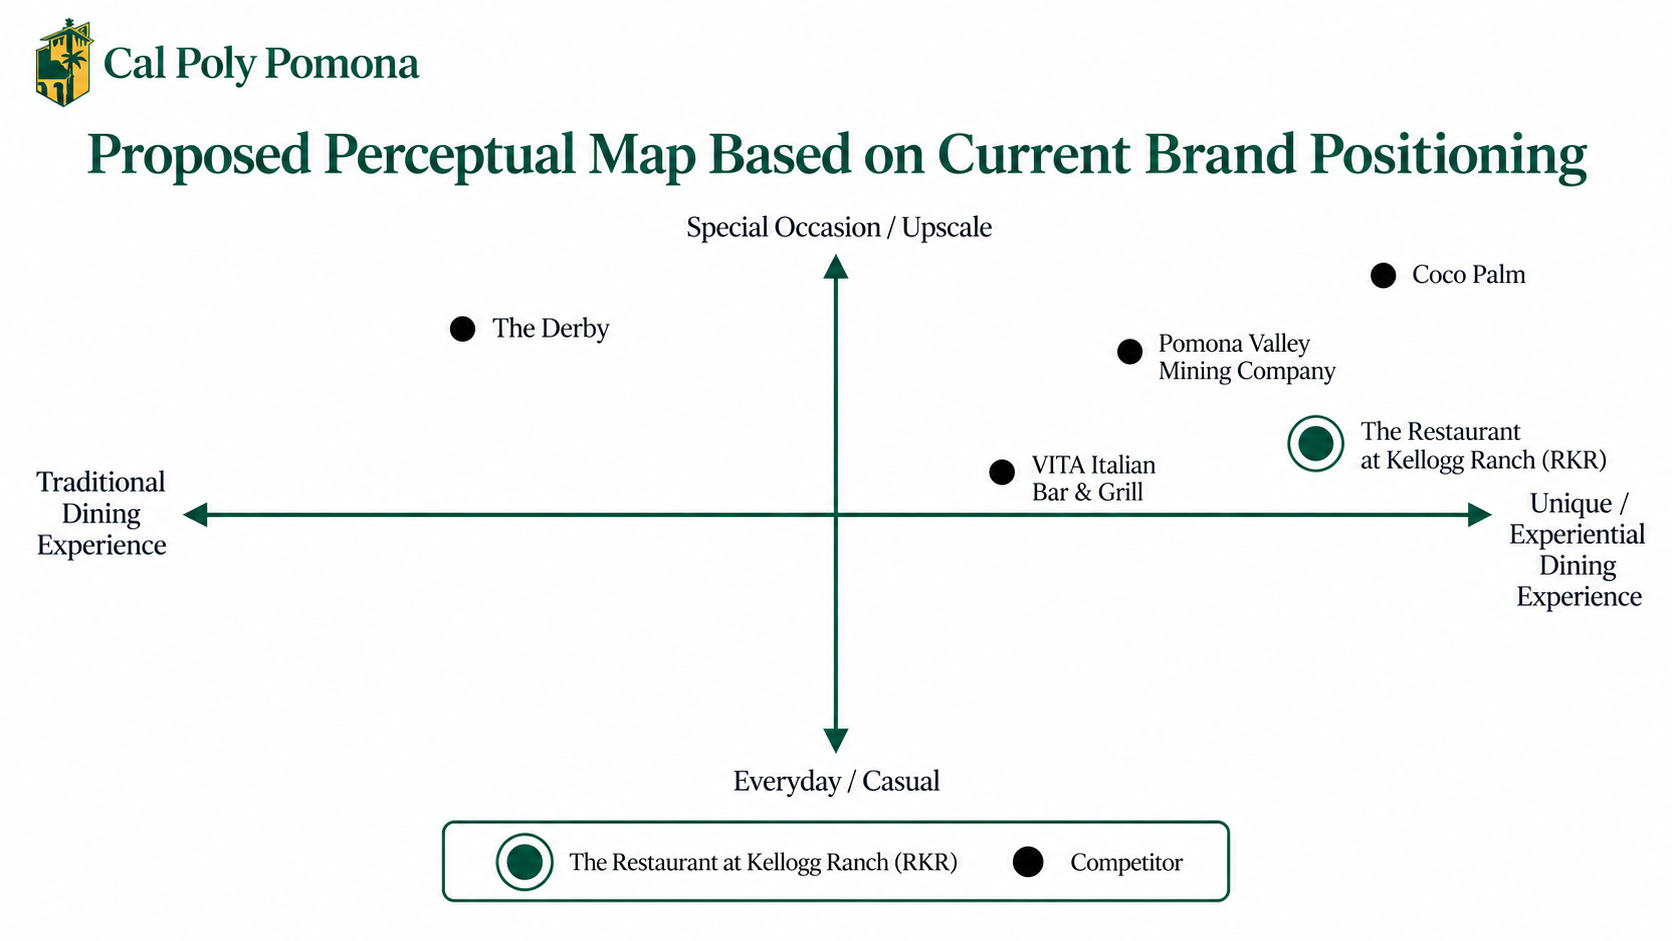
\includegraphics[keepaspectratio]{images/Cal Poly Pomona Perceptual Map.png}}

The reason for the RKR's current placement on the map is because its
student-operated setting and connection to CPP helps separate it from
its competitors that offer more traditional upscale dining experiences.
But, the map also reflects the team's assessment of each restaurant
based on its characteristics rather than customer feedback. Performing
more research could help our group determine how guests actually
perceive RKR and whether its current positioning on our map aligns with
those perceptions of the public.~

\subsubsection{Current Product/Services}\label{current-productservices}

The Restaurant at Kellogg Ranch (RKR) provides public lunch and dinner
service within a student-operated hospitality training restaurant at Cal
Poly Pomona. Its offering combines seasonal dining, student-delivered
service, and views of the campus. The website also promotes the
restaurant as a setting for business dinners, family celebrations, and
large parties or events. ({``The restaurant at kellogg ranch''} n.d.).

The published menus include starters, salads, sandwiches, entrées,
desserts, and beverages, with dietary options identified. (The
Restaurant at Kellogg Ranch n.d.b). Campus partnerships supply
ingredients and beverages, including produce from university farms,
campus-produced honey, Horsehill wines, and Innovation Brew Works beer.
These partnerships help distinguish RKR's offering through its
connection to Cal Poly Pomona and locally sourced food. (The Restaurant
at Kellogg Ranch n.d.a).

These characteristics directly support AO2, which compares guest ratings
of food quality, service quality, and atmosphere or physical
environment. Together, these dimensions represent the core experience
RKR provides. The restaurant's promotional descriptions establish what
it offers and emphasizes, while the planned post-visit survey will
assess how guests actually evaluate that experience. Seasonal dishes and
campus sourcing also provide potential content subjects for the
newsletter, Facebook, and Instagram work in AO1, AO3, and AO5.

\subsubsection{Current Pricing}\label{current-pricing}

RKR's published fall menus use individual item pricing. Lunch entrées
range from \$15 to \$23, while lunch sandwiches range from \$18 to \$20.
Individual dinner entrées range from \$16 to \$24, and a sirloin entrée
intended for two guests is listed at \$48. Desserts are priced at \$12
each. These amounts describe listed items rather than complete meal
totals. (The Restaurant at Kellogg Ranch n.d.b).

\begin{longtable}[]{@{}
  >{\raggedright\arraybackslash}p{(\linewidth - 2\tabcolsep) * \real{0.1800}}
  >{\raggedleft\arraybackslash}p{(\linewidth - 2\tabcolsep) * \real{0.2200}}@{}}
\toprule\noalign{}
\begin{minipage}[b]{\linewidth}\raggedright
Menu category
\end{minipage} & \begin{minipage}[b]{\linewidth}\raggedleft
Published price
\end{minipage} \\
\midrule\noalign{}
\endhead
\bottomrule\noalign{}
\endlastfoot
Lunch entrées & \$15--\$23 \\
Lunch sandwiches & \$18--\$20 \\
Individual dinner entrées & \$16--\$24 \\
Sirloin entrée for two & \$48 \\
Desserts & \$12 \\
Wine by the glass & \$6--\$10 \\
Beer & \$6--\$8 \\
\end{longtable}

Source: RKR's published fall menus (The Restaurant at Kellogg Ranch
n.d.b).

Pricing provides practical information prospective guests can use when
planning a visit. This relates to AO4 because finding the menu should
give visitors access to relevant dining information, including prices.
However, successful navigation does not establish that customers
consider those prices affordable or worthwhile. Price perceptions are
also outside AO2's primary comparison of food, service, and atmosphere.
The team should therefore describe current prices without claiming that
the project will determine an optimal pricing strategy. Pricing
rationale, discounts, and private-event rates require client
confirmation.

\subsubsection{Current Marketing
Channels}\label{current-marketing-channels}

RKR delivers its dining service directly through its campus restaurant
in Building 79 at 3801 West Temple Avenue in Pomona. Its contact page
provides location directions, telephone and email contact information,
and complimentary parking in Lot L with a reservation. Posted hours are
Monday through Friday, 11 a.m.--2 p.m., for lunch and Tuesday through
Friday, 5--8 p.m., for dinner, beginning August 24. (The Restaurant at
Kellogg Ranch n.d.c).

The website provides an OpenTable reservation widget, while walk-ins are
also welcome. ({``The restaurant at kellogg ranch''} n.d.). The team's
existing report identifies additional customer outreach through The
Collins Concierge newsletter, Facebook, and Instagram. These
communication channels can introduce guests to RKR and direct them
toward dining information or the reservation process.

This channel structure explains the relationship among the project's
AOs. AO1 examines newsletter clicks and attributed reservations; AO3
examines Facebook engagement and its association with OpenTable
activity; AO5 compares Instagram engagement across formats. AO4 examines
whether visitors can find the menu, identify hours, and reach the
reservation interface. These are distinct stages of the customer
journey. Reaching the reservation interface does not confirm a booking,
and reservation records alone do not capture walk-in visits.

\subsubsection{Current Integrated Marketing
Communications}\label{current-integrated-marketing-communications}

RKR's website emphasizes seasonal food, campus sourcing, hospitality
education, welcoming service, and scenic views. It includes guest
testimonials and directs visitors to
\href{https://www.instagram.com/rkr_cpp/}{RKR's Instagram account} for
team updates, seasonal menu changes, and special events. ({``The
restaurant at kellogg ranch''} n.d.). The sourcing page reinforces the
campus connection, while the ``Our Story'' page presents the
restaurant's educational origins and lists awards and recognitions. (The
Restaurant at Kellogg Ranch n.d.a; n.d.d).

The team's report also documents an RKR promotional section in The
Collins Concierge containing menu information, hours, and a reservation
link. It identifies Facebook and Instagram as additional channels under
investigation. Together, these activities provide several opportunities
to communicate the restaurant's offering and encourage a visit. However,
their presence does not establish that messaging, schedules, or
reservation links are coordinated across channels.

AO1, AO3, and AO5 address different aspects of communication
performance: newsletter design, Facebook content and messaging, and
Instagram formats. AO4 complements this work by assessing access to the
information and reservation interface that prospective guests need next.
The shared implication is that communication should be evaluated through
both audience response and subsequent actions where measurable. Higher
engagement alone should not be presented as evidence of increased
reservations. Client information about campaign planning, content
approval, and tracking is needed to assess the integration of RKR's
communications.

\subsection{Description of the Company's Current Digital Marketing
Practices}\label{description-of-the-companys-current-digital-marketing-practices}

\subsubsection{Brand Persona}\label{brand-persona}

\subsubsection{Digital Marketing
Channels/Medium}\label{digital-marketing-channelsmedium}

\paragraph{Website and Landing Page}\label{website-and-landing-page}

\paragraph{Keyword Research and SEO}\label{keyword-research-and-seo}

\paragraph{Email Marketing}\label{email-marketing}

\paragraph{Social Media Posting}\label{social-media-posting}

\paragraph{Paid Search Advertising}\label{paid-search-advertising}

\paragraph{Social Media Advertising}\label{social-media-advertising}

\paragraph{Display advertising}\label{display-advertising}

\subsubsection{Other digital marketing channels \&
tactics}\label{other-digital-marketing-channels-tactics}

\paragraph{Conversion Rate Optimization
(CRO)}\label{conversion-rate-optimization-cro}

\paragraph{Mobile Application}\label{mobile-application}

\paragraph{Affiliate Marketing}\label{affiliate-marketing}

\paragraph{Influencer Campaigns}\label{influencer-campaigns}

\subsubsection{Allocation of Resources to Customer-Influence
Efforts}\label{allocation-of-resources-to-customer-influence-efforts}

\paragraph{Demand Generation}\label{demand-generation}

\paragraph{Demand Harvesting}\label{demand-harvesting}

\paragraph{Loyalty Building}\label{loyalty-building}

\subsubsection{Analytics Infrastructure}\label{analytics-infrastructure}

\subsection{2.4 Competitive Analysis}\label{competitive-analysis}

RKR competes with restaurants in Pomona and the surrounding area.
Customers may compare food, prices, atmosphere, location, and available
dining times when choosing a restaurant. Our proposed comparisons are
Pomona Valley Mining Company, Coco Palm, The Derby, and VITA Italian Bar
\& Grill. We still need to confirm which restaurants RKR considers its
closest competitors.

\subsubsection{Industry Size}\label{industry-size}

The figures below describe the broader U.S. restaurant and foodservice
industry. They provide background for the project but do not measure the
size of RKR's local market.

\paragraph{Number of Companies}\label{number-of-companies}

We have not yet confirmed the number of restaurant companies in RKR's
local market. Before finding this number, our team needs to define the
area and types of restaurants included in the comparison. A count of
restaurant locations would also be different from a count of companies,
since one company may operate several locations.

\paragraph{Number of Employees}\label{number-of-employees}

The National Restaurant Association's initial 2026 forecast projected
total U.S. restaurant and foodservice employment of 15.8 million
people.\textsuperscript{5} This shows the size of the national industry,
but we have not yet obtained an employment estimate for RKR's local
market.

\paragraph{Annual Revenue and Key Financial
Information}\label{annual-revenue-and-key-financial-information}

The National Restaurant Association's initial forecast projected U.S.
restaurant and foodservice sales of \$1.55 trillion in
2026.\textsuperscript{5} In July, the association updated its expected
annual sales growth to 4.3\%, or 0.8\% after adjusting for inflation.
The update also reported uneven customer traffic and high operating
costs.\textsuperscript{6}

These conditions suggest that restaurants need to give customers a clear
reason to visit. For RKR, we think its student-run experience, seasonal
menus, and campus-grown ingredients could help communicate its
value.\textsuperscript{7} We have not obtained comparable annual revenue
figures for RKR and the selected competitors.

\paragraph{Existence of Dominant Players and
Competitors}\label{existence-of-dominant-players-and-competitors}

Our analysis focuses on restaurants that could appeal to customers
looking for a similar dining occasion. We have not established that any
of these restaurants dominates the local market.

Pomona Valley Mining Company and Coco Palm were selected as nearby
comparisons because both promote scenic dining.\textsuperscript{1,2} The
Derby in Arcadia provides a regional comparison for upscale dining and
special occasions.\textsuperscript{3} VITA Italian Bar \& Grill offers
another Pomona option and emphasizes Italian food, local ingredients,
and its dining atmosphere.\textsuperscript{4}

\begin{longtable}[]{@{}
  >{\raggedright\arraybackslash}p{(\linewidth - 6\tabcolsep) * \real{0.1800}}
  >{\raggedright\arraybackslash}p{(\linewidth - 6\tabcolsep) * \real{0.2200}}
  >{\raggedright\arraybackslash}p{(\linewidth - 6\tabcolsep) * \real{0.2400}}
  >{\raggedright\arraybackslash}p{(\linewidth - 6\tabcolsep) * \real{0.1800}}@{}}
\toprule\noalign{}
\begin{minipage}[b]{\linewidth}\raggedright
Restaurant
\end{minipage} & \begin{minipage}[b]{\linewidth}\raggedright
Main offering
\end{minipage} & \begin{minipage}[b]{\linewidth}\raggedright
Digital marketing features
\end{minipage} & \begin{minipage}[b]{\linewidth}\raggedright
What this means for RKR
\end{minipage} \\
\midrule\noalign{}
\endhead
\bottomrule\noalign{}
\endlastfoot
\textbf{RKR --- Pomona} & Student-run restaurant with seasonal food,
campus-grown ingredients, and hillside views.\textsuperscript{7} &
Website includes menus, visitor information, OpenTable reservations, and
an Instagram link.\textsuperscript{7} & Student involvement and campus
ingredients give RKR different topics to feature in its content. \\
\textbf{Pomona Valley Mining Company --- Pomona} & Hilltop dining,
Sunday brunch, and private events.\textsuperscript{1} & Website promotes
holiday meals and events, provides menu information, and links to
OpenTable reservations.\textsuperscript{1} & Competes for scenic dining
and celebrations. Its website connects promotions to a clear reservation
option. \\
\textbf{Coco Palm --- Pomona} & Cuban dining with city views and space
for special occasions.\textsuperscript{2} & Website provides menus,
reservations, online ordering, and event information.\textsuperscript{2}
& Offers another option for local customers looking for a meal with a
view or a celebration venue. \\
\textbf{The Derby --- Arcadia} & Upscale steakhouse with a long history
and a focus on its dining atmosphere.\textsuperscript{3} & Website
shares the restaurant's history, food and interior photos, reservation
links, and group-dining information.\textsuperscript{3} & Shows how a
restaurant can use its story and atmosphere to give customers a reason
to visit. \\
\textbf{VITA Italian Bar \& Grill --- Pomona} & Italian dining with
local ingredients, an outdoor terrace, and Sunday
brunch.\textsuperscript{4} & Website features menus, reservation links,
food photos, brunch promotions, and cooking classes.\textsuperscript{4}
& Provides another nearby dining option. Its food and event promotions
give us ideas for content RKR could test. \\
\end{longtable}

\emph{The table compares visible website features. It does not show
which restaurant has better marketing results.}

This comparison supports our analytics objectives by identifying content
and customer actions to evaluate. For AO5, we could compare Instagram
posts about food, students, and the dining atmosphere to see which
receive more engagement. The newsletter and website objectives could
examine whether menu information and reservation links encourage
customers to take the next step. Reservation-link clicks should be
measured separately from completed reservations.

\paragraph{Market Share of Each Major
Player}\label{market-share-of-each-major-player}

We have not found reliable market-share figures for RKR or the selected
competitors. Calculating revenue-based market share would require each
restaurant's sales and total sales for a clearly defined market during
the same period.

Because these figures are not available to our team, we cannot estimate
each restaurant's market share. Social media followers and online
reviews may help compare online visibility, but they do not measure
market share.

\subsubsection{Industry Outlook}\label{industry-outlook}

\paragraph{Industry Life Cycle}\label{industry-life-cycle}

\paragraph{Future Sales/Profit Growth
Outlook}\label{future-salesprofit-growth-outlook}

\subsubsection{Key Competitors and Their Digital Marketing
Strategies}\label{key-competitors-and-their-digital-marketing-strategies}

\paragraph{Target Market}\label{target-market}

\paragraph{Positioning}\label{positioning}

\paragraph{Website and Landing Page}\label{website-and-landing-page-1}

\paragraph{Keyword research and SEO}\label{keyword-research-and-seo-1}

\paragraph{Email Marketing Strategy}\label{email-marketing-strategy}

\paragraph{Social Media Posting}\label{social-media-posting-1}

\paragraph{Paid Search Advertising}\label{paid-search-advertising-1}

\paragraph{Social Media Advertising}\label{social-media-advertising-1}

\paragraph{Display Advertising}\label{display-advertising-1}

\paragraph{Conversion Rate Optimization
(CRO)}\label{conversion-rate-optimization-cro-1}

\paragraph{Mobile Application}\label{mobile-application-1}

\paragraph{Affiliate Marketing}\label{affiliate-marketing-1}

\paragraph{Influencer Campaigns}\label{influencer-campaigns-1}

\paragraph{Summary Table of
Comparison}\label{summary-table-of-comparison}

\subsection{Customer Analysis}\label{customer-analysis}

\subsubsection{Segments and Their Brief
Justification}\label{segments-and-their-brief-justification}

\paragraph{Segment A: Cal Poly Pomona Faculty and
Staff}\label{segment-a-cal-poly-pomona-faculty-and-staff}

This segment includes faculty, staff, and administrators who work on
campus. They are likely working adults with steady schedules and limited
time during the day. RKR's weekday lunch hours, from 11 a.m. to 2 p.m.,
fit their routine (The Restaurant at Kellogg Ranch n.d.c). These guests
may value convenience, a quality meal close to work, and a setting
suited for department lunches or meetings with colleagues. Many also
have a personal connection to the university and may want to support its
students. We expect this group to visit most often at lunch and to
return if the experience is consistent. The Collins Concierge already
reaches part of this audience, which makes it the most direct segment to
test through AO1.

\paragraph{Segment B: Cal Poly Pomona
Students}\label{segment-b-cal-poly-pomona-students}

This segment includes undergraduate and graduate students, including
hospitality students and their peers. Most are younger diners who are
active on social media. They may be more price-conscious than other
segments, since lunch entrées range from \$15 to \$23 (The Restaurant at
Kellogg Ranch n.d.b). On the other hand, RKR accepts Bronco Bucks, which
may make a visit easier to justify. Students may look for a social
outing, a special meal, or a place to bring visiting family. We expect
visits to be occasional and tied to events such as birthdays, family
visits, or graduation. Instagram is likely the strongest way to reach
this group, which connects to AO5.

\paragraph{Segment C: Local Professionals and Business
Groups}\label{segment-c-local-professionals-and-business-groups}

This segment includes employees of Pomona-area companies and
organizations who need a place for business meals. The RKR website
already promotes the restaurant for business dinners and large parties
({``The restaurant at kellogg ranch''} n.d.). These guests may value a
professional atmosphere, reliable service, and easy reservations. RKR's
farm-to-table menu and campus setting could also give business hosts a
unique place to bring clients. We expect this group to book in advance
and to dine in larger parties. However, RKR does not currently have a
confirmed channel that targets this group. The executive chef's LinkedIn
could help, but it is not an official RKR channel.

\paragraph{Segment D: Alumni and the Local
Community}\label{segment-d-alumni-and-the-local-community}

This segment includes Cal Poly Pomona alumni and residents of Pomona and
nearby cities. Alumni may feel loyalty to the university, while local
residents may be looking for something different from a typical night
out. Both groups may value the scenic views, seasonal menu, and
campus-grown ingredients (The Restaurant at Kellogg Ranch n.d.a). We
expect this segment to visit for celebrations such as birthdays,
anniversaries, and family gatherings. Notably, this segment compares RKR
most directly with Pomona Valley Mining Company and Coco Palm, which
also promote scenic dining. RKR does not offer weekend service, which
may limit visits from guests who celebrate on Saturdays or Sundays (The
Restaurant at Kellogg Ranch n.d.c).

\paragraph{\texorpdfstring{\textbf{Summary Table of
Segments}}{Summary Table of Segments}}\label{summary-table-of-segments}

\begin{longtable}[]{@{}
  >{\raggedright\arraybackslash}p{(\linewidth - 8\tabcolsep) * \real{0.1800}}
  >{\raggedright\arraybackslash}p{(\linewidth - 8\tabcolsep) * \real{0.2200}}
  >{\raggedright\arraybackslash}p{(\linewidth - 8\tabcolsep) * \real{0.2400}}
  >{\raggedright\arraybackslash}p{(\linewidth - 8\tabcolsep) * \real{0.1800}}
  >{\raggedright\arraybackslash}p{(\linewidth - 8\tabcolsep) * \real{0.1800}}@{}}
\toprule\noalign{}
\begin{minipage}[b]{\linewidth}\raggedright
Characteristic
\end{minipage} & \begin{minipage}[b]{\linewidth}\raggedright
Segment A: Faculty and Staff
\end{minipage} & \begin{minipage}[b]{\linewidth}\raggedright
Segment B: Students
\end{minipage} & \begin{minipage}[b]{\linewidth}\raggedright
Segment C: Local Professionals
\end{minipage} & \begin{minipage}[b]{\linewidth}\raggedright
Segment D: Alumni and Local Community
\end{minipage} \\
\midrule\noalign{}
\endhead
\bottomrule\noalign{}
\endlastfoot
\textbf{Demographics} & Working adults employed on campus &
Undergraduate and graduate students & Employees of Pomona-area companies
& Alumni and residents of Pomona and nearby cities \\
\textbf{Psychographics} & Busy, connected to the university, supportive
of students & Social, active online, budget-aware & Professional,
focused on impressions and reliability & Loyal to CPP or looking for a
unique local experience \\
\textbf{Benefits sought} & Convenience, quality lunch, meeting space &
Social outing, special occasion meal, value & Professional setting,
dependable service, easy booking & Scenic views, seasonal food, a
memorable celebration \\
\textbf{Behavioral patterns} & Frequent weekday lunch visits &
Occasional, event-driven visits & Advance bookings for larger parties &
Special-occasion visits, often on evenings \\
\textbf{Likely channels} & The Collins Concierge, campus email &
Instagram, Facebook & Website, Google, LinkedIn & Instagram, Facebook,
Google, Yelp, alumni outreach \\
\end{longtable}

\subsubsection{Segment Analysis}\label{segment-analysis}

Each segment was evaluated on four criteria. Identifiability is whether
the group can be clearly defined and measured. Actionability is whether
RKR can serve the group with its current menu, hours, and resources.
Substantiality is whether the group is large enough or spends enough to
support demand. Accessibility is whether RKR can reach the group through
its existing channels.

Faculty and staff rate highest overall. They are easy to identify, they
are on campus during lunch hours, and the Concierge newsletter already
reaches part of this group. Their total size is still unknown, so
substantiality is rated medium until reservation data can confirm it.

Students are easy to identify and reach through Instagram. On the other
hand, menu prices may limit how often they visit, and their spending per
visit is likely lower than other segments. As such, students rate lower
on actionability and substantiality.

Local professionals fit the business dining the website already
promotes. However, RKR has no official channel aimed at this group, and
its size in the Pomona area has not been measured. This makes
accessibility the weakest point for this segment.

Alumni and the local community are a large potential audience with clear
reasons to visit. RKR can reach them through social media and review
sites, but competition for scenic and special-occasion dining is strong.
The lack of weekend service also limits how well RKR can serve them.

\paragraph{\texorpdfstring{\textbf{Summary Table of Segment
Evaluation}}{Summary Table of Segment Evaluation}}\label{summary-table-of-segment-evaluation}

\begin{longtable}[]{@{}
  >{\raggedright\arraybackslash}p{(\linewidth - 8\tabcolsep) * \real{0.1800}}
  >{\raggedright\arraybackslash}p{(\linewidth - 8\tabcolsep) * \real{0.2200}}
  >{\raggedright\arraybackslash}p{(\linewidth - 8\tabcolsep) * \real{0.2400}}
  >{\raggedright\arraybackslash}p{(\linewidth - 8\tabcolsep) * \real{0.1800}}
  >{\raggedright\arraybackslash}p{(\linewidth - 8\tabcolsep) * \real{0.1800}}@{}}
\toprule\noalign{}
\begin{minipage}[b]{\linewidth}\raggedright
Criterion
\end{minipage} & \begin{minipage}[b]{\linewidth}\raggedright
Segment A: Faculty and Staff
\end{minipage} & \begin{minipage}[b]{\linewidth}\raggedright
Segment B: Students
\end{minipage} & \begin{minipage}[b]{\linewidth}\raggedright
Segment C: Local Professionals
\end{minipage} & \begin{minipage}[b]{\linewidth}\raggedright
Segment D: Alumni and Local Community
\end{minipage} \\
\midrule\noalign{}
\endhead
\bottomrule\noalign{}
\endlastfoot
\textbf{Identifiability} & High & High & Medium & Medium \\
\textbf{Actionability} & High & Medium & Medium & Medium \\
\textbf{Substantiality} & Medium & Medium & Medium & High \\
\textbf{Accessibility} & High & High & Low & Medium \\
\textbf{Overall attractiveness} & High & Medium & Low to Medium & Medium
to High \\
\end{longtable}

Based on this evaluation, faculty and staff are the most attractive
primary target. This segment fits RKR's weekday hours, is reachable
through channels RKR already uses, and can be measured directly through
AO1. Alumni and the local community are recommended as a secondary
target because of their size and their interest in celebration dining.
Reaching them will depend on stronger social media content, which AO3
and AO5 will help evaluate. These choices are based on our team's
assessment and should be confirmed with OpenTable reservation data and
AO2 survey responses.

\subsection{SWOT Analysis}\label{swot-analysis}

\subsubsection{Strengths}\label{strengths}

\subsubsection{Weaknesses}\label{weaknesses}

\subsubsection{Opportunities}\label{opportunities}

\subsubsection{Threats}\label{threats}

\subsubsection{\texorpdfstring{\textbf{Summary: SWOT
quadrants}}{Summary: SWOT quadrants}}\label{summary-swot-quadrants}

\subsection*{References}\label{references}
\addcontentsline{toc}{subsection}{References}

\phantomsection\label{refs}
\begin{CSLReferences}{1}{0}
\begin{enumerate}
\def\labelenumi{\arabic{enumi}.}
\item
  Pomona Valley Mining Co.~Pomona Valley Mining Co.~Accessed October 11,
  2026. \url{https://www.pomonavalleyminingco.com/}
\item
  Coco Palm Restaurant. Coco Palm Restaurant. Accessed October 11, 2026.
  \url{https://www.cocopalmrestaurant.com/}
\item
  The Derby. The Derby. Accessed October 11, 2026.
  \url{https://www.thederbyarcadia.com/}
\item
  VITA Italian Bar \& Grill. VITA Italian Bar \& Grill. Accessed October
  11, 2026. \url{https://www.vitalosangeles.com/}
\item
  National Restaurant Association. State of the restaurant industry
  2026. Published February 11, 2026. Accessed October 11, 2026.
  \url{https://restaurant.org/research-and-media/research/research-reports/state-of-the-industry/}
\item
  National Restaurant Association. Restaurants remain resilient despite
  challenging business conditions. Published July 22, 2026. Accessed
  October 11, 2026.
  \url{https://restaurant.org/research-and-media/research/restaurant-economic-insights/analysis-commentary/restaurants-remain-resilient-despite-challenging-business-conditions/}
\item
  California State Polytechnic University, Pomona. The Restaurant at
  Kellogg Ranch. Accessed October 11, 2026.
  \url{https://www.cpp.edu/rkr/}
\end{enumerate}

\bibitem[\citeproctext]{ref-arora2006}
Arora, Raj and Joe Singer (2006),
{``\href{https://doi.org/10.1300/J396v28n01_05}{Customer satisfaction
and value as drivers of business success for fine dining
restaurants},''} \emph{Services Marketing Quarterly}, 28 (1), 89--102.

\bibitem[\citeproctext]{ref-bashirzadeh2022}
Bashirzadeh, Yashar, Robert Mai, and Corinne Faure (2022),
{``\href{https://doi.org/10.1016/j.ijresmar.2021.06.008}{How rich is too
rich? Visual design elements in digital marketing communications},''}
\emph{International Journal of Research in Marketing}, 39 (1), 58--76.

\bibitem[\citeproctext]{ref-bicudodecastro2025}
Bicudo De Castro, Vicente (2025),
{``\href{https://doi.org/10.1080/07294360.2025.2510662}{Quantifying the
burden of organisational bulk emails in a business school},''}
\emph{Higher Education Research \& Development}, 44 (8), 1934--48.

\bibitem[\citeproctext]{ref-bushara2023}
Bushara, Meimona Abdelrhim, Ahmed Hassan Abdou, Thowayeb H. Hassan, Abu
Elnasr E. Sobaih, Abdullah Saleh Mohammed Albohnayh, Waleed Ghazi
Alshammari, Mohammed Aldoreeb, Ahmed Anwar Elsaed, and Mohamed Ahmed
Elsaied (2023), {``\href{https://doi.org/10.3390/su15065331}{Power of
Social Media Marketing: How Perceived Value Mediates the Impact on
Restaurant Followers{'} Purchase Intention, Willingness to Pay a Premium
Price, and E-WoM?}''} \emph{Sustainability}, 15 (6), 5331.

\bibitem[\citeproctext]{ref-collins_rkr}
California State Polytechnic University, Pomona (n.d.), {``The
restaurant at kellogg ranch,''} The Collins College of Hospitality
Management, (accessed October 11, 2026), {[}available at
\url{https://www.cpp.edu/collins/academic-programs/the-restaurant-at-kellogg-ranch.shtml}{]}.

\bibitem[\citeproctext]{ref-davis1989}
Davis, Fred D. (1989),
{``\href{https://doi.org/10.2307/249008}{Perceived usefulness, perceived
ease of use, and user acceptance of information technology},''}
\emph{MIS Quarterly}, 13 (3), 319--40.

\bibitem[\citeproctext]{ref-dedeke2016}
Dedeke, Adenekan Nick (2016),
{``\href{https://doi.org/10.1016/j.tourman.2016.01.001}{Travel web-site
design: Information task-fit, service quality and purchase
intention},''} \emph{Tourism Management}, 54, 541--54.

\bibitem[\citeproctext]{ref-delone2003}
DeLone, William H. and Ephraim R. McLean (2003),
{``\href{https://doi.org/10.1080/07421222.2003.11045748}{The {DeLone}
and {McLean} model of information systems success: A ten-year
update},''} \emph{Journal of Management Information Systems}, 19 (4),
9--30.

\bibitem[\citeproctext]{ref-go2024}
Go, Sydney (2024),
{``\href{https://www.semrush.com/blog/email-marketing}{What Is Email
Marketing? The Definitive Guide for Beginners}.''}

\bibitem[\citeproctext]{ref-halloran2021}
Halloran, Timothy J. and Richard J. Lutz (2021),
{``\href{https://doi.org/10.1016/j.intmar.2021.05.003}{Let's Give Them
Something to Talk About: Which Social Media Engagements Predict Purchase
Frequency?}''} \emph{Journal of Interactive Marketing}, 56 (1), 83--95.

\bibitem[\citeproctext]{ref-han2009}
Han, Heesup and Kisang Ryu (2009),
{``\href{https://doi.org/10.1177/1096348009344212}{The roles of the
physical environment, price perception, and customer satisfaction in
determining customer loyalty in the restaurant industry},''}
\emph{Journal of Hospitality \& Tourism Research}, 33 (4), 487--510.

\bibitem[\citeproctext]{ref-hanaysha2022}
Hanaysha, Jalal Rajeh (2022),
{``\href{https://doi.org/10.1108/BFJ-08-2021-0907}{An examination of
social media advertising features, brand engagement and purchase
intention in the fast food industry},''} \emph{British Food Journal},
124 (11), 4143--60.

\bibitem[\citeproctext]{ref-hartemo2016}
Hartemo, Mari, Reima Suomi, and Ulla Hakala (2016),
{``\href{https://doi.org/10.4018/JECO.2016070101}{Towards improved
performance: A model for testing email newsletter design},''}
\emph{Journal of Electronic Commerce in Organizations}, 14 (3), 1--16.

\bibitem[\citeproctext]{ref-heung2012}
Heung, Vincent C. S. and Tianming Gu (2012),
{``\href{https://doi.org/10.1016/j.ijhm.2012.02.004}{Influence of
restaurant atmospherics on patron satisfaction and behavioral
intentions},''} \emph{International Journal of Hospitality Management},
31 (4), 1167--77.

\bibitem[\citeproctext]{ref-hornbaek2006}
Hornbæk, Kasper (2006),
{``\href{https://doi.org/10.1016/j.ijhcs.2005.06.002}{Current practice
in measuring usability: Challenges to usability studies and
research},''} \emph{International Journal of Human-Computer Studies}, 64
(2), 79--102.

\bibitem[\citeproctext]{ref-hornbaeklaw2007}
Hornbæk, Kasper and Effie Lai-Chong Law (2007),
{``\href{https://doi.org/10.1145/1240624.1240722}{Meta-analysis of
correlations among usability measures},''} in \emph{Proceedings of the
SIGCHI conference on human factors in computing systems}, Association
for Computing Machinery, 617--26.

\bibitem[\citeproctext]{ref-jeong2001}
Jeong, Miyoung and Carolyn U. Lambert (2001),
{``\href{https://doi.org/10.1016/S0278-4319(00)00041-4}{Adaptation of an
information quality framework to measure customers' behavioral
intentions to use lodging web sites},''} \emph{International Journal of
Hospitality Management}, 20 (2), 129--46.

\bibitem[\citeproctext]{ref-jones2023}
Jones, Alexandra (2023),
{``\href{https://www.opentable.com/restaurant-solutions/resources/email-marketing-restaurants/}{The
complete restaurant email marketing guide}.''}

\bibitem[\citeproctext]{ref-kim2012}
Kim, Hak-Seon, Kwang-Woo Lee, Dong-Soo Lee, Hyun-Woo Joung, and Jingxue
Jessica Yuan (2012),
{``\href{https://doi.org/10.1080/1528008X.2012.692278}{Assessing the
quality of a restaurant's website using DINEWEBQUAL},''} \emph{Journal
of Quality Assurance in Hospitality \& Tourism}, 13 (3), 235--45.

\bibitem[\citeproctext]{ref-kong2021}
Kong, Ruoyan, Haiyi Zhu, and Joseph A. Konstan (2021),
{``\href{https://doi.org/10.1145/3449154}{Learning to Ignore: A Case
Study of Organization-Wide Bulk Email Effectiveness},''}
\emph{Proceedings of the ACM on Human-Computer Interaction}, 5 (CSCW1),
1--23.

\bibitem[\citeproctext]{ref-kulikovskaja2023}
Kulikovskaja, Viktorija, Marco Hubert, Klaus G. Grunert, and Hong Zhao
(2023),
{``\href{https://doi.org/10.1016/j.jretconser.2023.103445}{Driving
marketing outcomes through social media-based customer engagement},''}
\emph{Journal of Retailing and Consumer Services}, 74, 103445.

\bibitem[\citeproctext]{ref-kumar2021}
Kumar, Ashish (2021),
{``\href{https://doi.org/10.1016/j.jretconser.2020.102349}{An empirical
examination of the effects of design elements of email newsletters on
consumers{'} email responses and their purchase},''} \emph{Journal of
Retailing and Consumer Services}, 58, 102349.

\bibitem[\citeproctext]{ref-kumar2018}
Kumar, Ashish and Jari Salo (2018),
{``\href{https://doi.org/10.1080/13527266.2016.1147485}{Effects of link
placements in email newsletters on their click-through rate.}''}
\emph{Journal of Marketing Communications}, 24 (5), 535--48.

\bibitem[\citeproctext]{ref-kwok2026}
Kwok, Linchi (2026), {``Building sustainable demand for the restaurant
at kellogg ranch: A data-driven brand, content, and digital marketing
initiative.''}

\bibitem[\citeproctext]{ref-lee2026}
Lee, Seonjeong (Ally) and Soo Yeon Kwak (2026),
{``\href{https://doi.org/10.1016/j.ijhm.2026.104713}{Enhancing customer
inspiration and engagement experiences on restaurant social media},''}
\emph{International Journal of Hospitality Management}, 138, 104713.

\bibitem[\citeproctext]{ref-manningham2024}
Manningham, Daphnée, Hugo Asselin, and Benoit Bourguignon (2024),
{``\href{https://doi.org/10.3390/tourhosp5020020}{Be Direct! Restaurant
Social Media Posts to Drive Customer Engagement in Times of Crisis and
Beyond},''} \emph{Tourism and Hospitality}, 5 (2), 304--13.

\bibitem[\citeproctext]{ref-namkung2007}
Namkung, Young and SooCheong Jang (2007),
{``\href{https://doi.org/10.1177/1096348007299924}{Does food quality
really matter in restaurants? Its impact on customer satisfaction and
behavioral intentions},''} \emph{Journal of Hospitality \& Tourism
Research}, 31 (3), 387--409.

\bibitem[\citeproctext]{ref-philp2022}
Philp, Matthew, Jenna Jacobson, and Ethan Pancer (2022b),
{``\href{https://doi.org/10.1016/j.jbusres.2022.05.078}{Predicting
social media engagement with computer vision: An examination of food
marketing on Instagram},''} \emph{Journal of Business Research}, 149,
736--47.

\bibitem[\citeproctext]{ref-philp2022a}
Philp, Matthew, Jenna Jacobson, and Ethan Pancer (2022a),
{``\href{https://doi.org/10.1016/j.jbusres.2022.05.078}{Predicting
social media engagement with computer vision: An examination of food
marketing on Instagram},''} \emph{Journal of Business Research}, 149,
736--47.

\bibitem[\citeproctext]{ref-ryu2012}
Ryu, Kisang, Hye-Rin Lee, and Woo Gon Kim (2012),
{``\href{https://doi.org/10.1108/09596111211206141}{The influence of the
quality of the physical environment, food, and service on restaurant
image, customer perceived value, customer satisfaction, and behavioral
intentions},''} \emph{International Journal of Contemporary Hospitality
Management}, 24 (2), 200--223.

\bibitem[\citeproctext]{ref-skourou2024}
Skourou, Evangelia and Dimitris Spiliotopoulos (2024),
{``\href{https://doi.org/10.3390/mti8100087}{Assessment of purchasing
influence of email campaigns using eye tracking},''} \emph{Multimodal
Technologies and Interaction}, 8 (10), 87.

\bibitem[\citeproctext]{ref-therest}
{``\href{https://www.cpp.edu/rkr/}{The restaurant at kellogg ranch}''}
(n.d.).

\bibitem[\citeproctext]{ref-rkr_menu}
The Restaurant at Kellogg Ranch (n.d.b), {``Our menu,''} California
State Polytechnic University, Pomona, (accessed October 11, 2026),
{[}available at \url{https://www.cpp.edu/rkr/menu.shtml}{]}.

\bibitem[\citeproctext]{ref-rkr_sourcing}
The Restaurant at Kellogg Ranch (n.d.a), {``Locally sourced food,''}
California State Polytechnic University, Pomona, (accessed October 11,
2026), {[}available at
\url{https://www.cpp.edu/rkr/locally-sourced-food.shtml}{]}.

\bibitem[\citeproctext]{ref-rkr_contact}
The Restaurant at Kellogg Ranch (n.d.c), {``Contact us,''} California
State Polytechnic University, Pomona, (accessed October 11, 2026),
{[}available at \url{https://www.cpp.edu/rkr/contact-us.shtml}{]}.

\bibitem[\citeproctext]{ref-rkr_story}
The Restaurant at Kellogg Ranch (n.d.d), {``Our story,''} California
State Polytechnic University, Pomona, (accessed October 11, 2026),
{[}available at \url{https://www.cpp.edu/rkr/our-story.shtml}{]}.

\bibitem[\citeproctext]{ref-tuch2012}
Tuch, Alexandre N., Sandra P. Roth, Kasper Hornbæk, Klaus Opwis, and
Javier A. Bargas-Avila (2012),
{``\href{https://doi.org/10.1016/j.chb.2012.03.024}{Is beautiful really
usable? Toward understanding the relation between usability, aesthetics,
and affect in HCI},''} \emph{Computers in Human Behavior}, 28 (5),
1596--1607.

\bibitem[\citeproctext]{ref-veloso2023}
Veloso, Mónica and Monica Gomez-Suarez (2023),
{``\href{https://doi.org/10.1108/JHTT-08-2021-0241}{The influential role
of hotel-generated content on social media},''} \emph{Journal of
Hospitality and Tourism Technology}, 14 (2), 245--57.

\bibitem[\citeproctext]{ref-yost2021}
Yost, Elizabeth, Tingting Zhang, and Ruoxi Qi (2021),
{``\href{https://doi.org/10.1016/j.jhtm.2020.10.008}{The power of
engagement: Understanding active social media engagement and the impact
on sales in the hospitality industry},''} \emph{Journal of Hospitality
and Tourism Management}, 46, 83--95.

\bibitem[\citeproctext]{ref-zunac2022}
Zunac, Ana Globocnik, Lana Miletic, and Goran Kozina (2022),
{``\href{https://www.proquest.com/docview/2735560511/abstract/A22D6AB6B6984192PQ/10}{Self-sufficiency
of e-mail as a marketing tool},''} Varazdin, Croatia: Varazdin
Development; Entrepreneurship Agency (VADEA), 147--53.

\end{CSLReferences}




\end{document}
